% Options for packages loaded elsewhere
\PassOptionsToPackage{unicode}{hyperref}
\PassOptionsToPackage{hyphens}{url}
\PassOptionsToPackage{dvipsnames,svgnames,x11names}{xcolor}
%
\documentclass[
]{article}

\usepackage{amsmath,amssymb}
\usepackage{lmodern}
\usepackage{iftex}
\ifPDFTeX
  \usepackage[T1]{fontenc}
  \usepackage[utf8]{inputenc}
  \usepackage{textcomp} % provide euro and other symbols
\else % if luatex or xetex
  \usepackage{unicode-math}
  \defaultfontfeatures{Scale=MatchLowercase}
  \defaultfontfeatures[\rmfamily]{Ligatures=TeX,Scale=1}
\fi
% Use upquote if available, for straight quotes in verbatim environments
\IfFileExists{upquote.sty}{\usepackage{upquote}}{}
\IfFileExists{microtype.sty}{% use microtype if available
  \usepackage[]{microtype}
  \UseMicrotypeSet[protrusion]{basicmath} % disable protrusion for tt fonts
}{}
\makeatletter
\@ifundefined{KOMAClassName}{% if non-KOMA class
  \IfFileExists{parskip.sty}{%
    \usepackage{parskip}
  }{% else
    \setlength{\parindent}{0pt}
    \setlength{\parskip}{6pt plus 2pt minus 1pt}}
}{% if KOMA class
  \KOMAoptions{parskip=half}}
\makeatother
\usepackage{xcolor}
\usepackage[top=30mm,left=30mm,right=20mm,bottom=20mm]{geometry}
\setlength{\emergencystretch}{3em} % prevent overfull lines
\setcounter{secnumdepth}{-\maxdimen} % remove section numbering
% Make \paragraph and \subparagraph free-standing
\ifx\paragraph\undefined\else
  \let\oldparagraph\paragraph
  \renewcommand{\paragraph}[1]{\oldparagraph{#1}\mbox{}}
\fi
\ifx\subparagraph\undefined\else
  \let\oldsubparagraph\subparagraph
  \renewcommand{\subparagraph}[1]{\oldsubparagraph{#1}\mbox{}}
\fi

\usepackage{color}
\usepackage{fancyvrb}
\newcommand{\VerbBar}{|}
\newcommand{\VERB}{\Verb[commandchars=\\\{\}]}
\DefineVerbatimEnvironment{Highlighting}{Verbatim}{commandchars=\\\{\}}
% Add ',fontsize=\small' for more characters per line
\usepackage{framed}
\definecolor{shadecolor}{RGB}{241,243,245}
\newenvironment{Shaded}{\begin{snugshade}}{\end{snugshade}}
\newcommand{\AlertTok}[1]{\textcolor[rgb]{0.68,0.00,0.00}{#1}}
\newcommand{\AnnotationTok}[1]{\textcolor[rgb]{0.37,0.37,0.37}{#1}}
\newcommand{\AttributeTok}[1]{\textcolor[rgb]{0.40,0.45,0.13}{#1}}
\newcommand{\BaseNTok}[1]{\textcolor[rgb]{0.68,0.00,0.00}{#1}}
\newcommand{\BuiltInTok}[1]{\textcolor[rgb]{0.00,0.23,0.31}{#1}}
\newcommand{\CharTok}[1]{\textcolor[rgb]{0.13,0.47,0.30}{#1}}
\newcommand{\CommentTok}[1]{\textcolor[rgb]{0.37,0.37,0.37}{#1}}
\newcommand{\CommentVarTok}[1]{\textcolor[rgb]{0.37,0.37,0.37}{\textit{#1}}}
\newcommand{\ConstantTok}[1]{\textcolor[rgb]{0.56,0.35,0.01}{#1}}
\newcommand{\ControlFlowTok}[1]{\textcolor[rgb]{0.00,0.23,0.31}{#1}}
\newcommand{\DataTypeTok}[1]{\textcolor[rgb]{0.68,0.00,0.00}{#1}}
\newcommand{\DecValTok}[1]{\textcolor[rgb]{0.68,0.00,0.00}{#1}}
\newcommand{\DocumentationTok}[1]{\textcolor[rgb]{0.37,0.37,0.37}{\textit{#1}}}
\newcommand{\ErrorTok}[1]{\textcolor[rgb]{0.68,0.00,0.00}{#1}}
\newcommand{\ExtensionTok}[1]{\textcolor[rgb]{0.00,0.23,0.31}{#1}}
\newcommand{\FloatTok}[1]{\textcolor[rgb]{0.68,0.00,0.00}{#1}}
\newcommand{\FunctionTok}[1]{\textcolor[rgb]{0.28,0.35,0.67}{#1}}
\newcommand{\ImportTok}[1]{\textcolor[rgb]{0.00,0.46,0.62}{#1}}
\newcommand{\InformationTok}[1]{\textcolor[rgb]{0.37,0.37,0.37}{#1}}
\newcommand{\KeywordTok}[1]{\textcolor[rgb]{0.00,0.23,0.31}{#1}}
\newcommand{\NormalTok}[1]{\textcolor[rgb]{0.00,0.23,0.31}{#1}}
\newcommand{\OperatorTok}[1]{\textcolor[rgb]{0.37,0.37,0.37}{#1}}
\newcommand{\OtherTok}[1]{\textcolor[rgb]{0.00,0.23,0.31}{#1}}
\newcommand{\PreprocessorTok}[1]{\textcolor[rgb]{0.68,0.00,0.00}{#1}}
\newcommand{\RegionMarkerTok}[1]{\textcolor[rgb]{0.00,0.23,0.31}{#1}}
\newcommand{\SpecialCharTok}[1]{\textcolor[rgb]{0.37,0.37,0.37}{#1}}
\newcommand{\SpecialStringTok}[1]{\textcolor[rgb]{0.13,0.47,0.30}{#1}}
\newcommand{\StringTok}[1]{\textcolor[rgb]{0.13,0.47,0.30}{#1}}
\newcommand{\VariableTok}[1]{\textcolor[rgb]{0.07,0.07,0.07}{#1}}
\newcommand{\VerbatimStringTok}[1]{\textcolor[rgb]{0.13,0.47,0.30}{#1}}
\newcommand{\WarningTok}[1]{\textcolor[rgb]{0.37,0.37,0.37}{\textit{#1}}}

\providecommand{\tightlist}{%
  \setlength{\itemsep}{0pt}\setlength{\parskip}{0pt}}\usepackage{longtable,booktabs,array}
\usepackage{calc} % for calculating minipage widths
% Correct order of tables after \paragraph or \subparagraph
\usepackage{etoolbox}
\makeatletter
\patchcmd\longtable{\par}{\if@noskipsec\mbox{}\fi\par}{}{}
\makeatother
% Allow footnotes in longtable head/foot
\IfFileExists{footnotehyper.sty}{\usepackage{footnotehyper}}{\usepackage{footnote}}
\makesavenoteenv{longtable}
\usepackage{graphicx}
\makeatletter
\def\maxwidth{\ifdim\Gin@nat@width>\linewidth\linewidth\else\Gin@nat@width\fi}
\def\maxheight{\ifdim\Gin@nat@height>\textheight\textheight\else\Gin@nat@height\fi}
\makeatother
% Scale images if necessary, so that they will not overflow the page
% margins by default, and it is still possible to overwrite the defaults
% using explicit options in \includegraphics[width, height, ...]{}
\setkeys{Gin}{width=\maxwidth,height=\maxheight,keepaspectratio}
% Set default figure placement to htbp
\makeatletter
\def\fps@figure{htbp}
\makeatother
\newlength{\cslhangindent}
\setlength{\cslhangindent}{1.5em}
\newlength{\csllabelwidth}
\setlength{\csllabelwidth}{3em}
\newlength{\cslentryspacingunit} % times entry-spacing
\setlength{\cslentryspacingunit}{\parskip}
\newenvironment{CSLReferences}[2] % #1 hanging-ident, #2 entry spacing
 {% don't indent paragraphs
  \setlength{\parindent}{0pt}
  % turn on hanging indent if param 1 is 1
  \ifodd #1
  \let\oldpar\par
  \def\par{\hangindent=\cslhangindent\oldpar}
  \fi
  % set entry spacing
  \setlength{\parskip}{#2\cslentryspacingunit}
 }%
 {}
\usepackage{calc}
\newcommand{\CSLBlock}[1]{#1\hfill\break}
\newcommand{\CSLLeftMargin}[1]{\parbox[t]{\csllabelwidth}{#1}}
\newcommand{\CSLRightInline}[1]{\parbox[t]{\linewidth - \csllabelwidth}{#1}\break}
\newcommand{\CSLIndent}[1]{\hspace{\cslhangindent}#1}

\makeatletter
\makeatother
\makeatletter
\makeatother
\makeatletter
\@ifpackageloaded{caption}{}{\usepackage{caption}}
\AtBeginDocument{%
\ifdefined\contentsname
  \renewcommand*\contentsname{Table of contents}
\else
  \newcommand\contentsname{Table of contents}
\fi
\ifdefined\listfigurename
  \renewcommand*\listfigurename{List of Figures}
\else
  \newcommand\listfigurename{List of Figures}
\fi
\ifdefined\listtablename
  \renewcommand*\listtablename{List of Tables}
\else
  \newcommand\listtablename{List of Tables}
\fi
\ifdefined\figurename
  \renewcommand*\figurename{Figure}
\else
  \newcommand\figurename{Figure}
\fi
\ifdefined\tablename
  \renewcommand*\tablename{Table}
\else
  \newcommand\tablename{Table}
\fi
}
\@ifpackageloaded{float}{}{\usepackage{float}}
\floatstyle{ruled}
\@ifundefined{c@chapter}{\newfloat{codelisting}{h}{lop}}{\newfloat{codelisting}{h}{lop}[chapter]}
\floatname{codelisting}{Listing}
\newcommand*\listoflistings{\listof{codelisting}{List of Listings}}
\makeatother
\makeatletter
\@ifpackageloaded{caption}{}{\usepackage{caption}}
\@ifpackageloaded{subcaption}{}{\usepackage{subcaption}}
\makeatother
\makeatletter
\@ifpackageloaded{tcolorbox}{}{\usepackage[many]{tcolorbox}}
\makeatother
\makeatletter
\@ifundefined{shadecolor}{\definecolor{shadecolor}{rgb}{.97, .97, .97}}
\makeatother
\makeatletter
\makeatother
\ifLuaTeX
  \usepackage{selnolig}  % disable illegal ligatures
\fi
\IfFileExists{bookmark.sty}{\usepackage{bookmark}}{\usepackage{hyperref}}
\IfFileExists{xurl.sty}{\usepackage{xurl}}{} % add URL line breaks if available
\urlstyle{same} % disable monospaced font for URLs
\hypersetup{
  pdftitle={Estimação},
  colorlinks=true,
  linkcolor={blue},
  filecolor={Maroon},
  citecolor={Blue},
  urlcolor={Blue},
  pdfcreator={LaTeX via pandoc}}

\title{Estimação}
\author{}
\date{}

\begin{document}
\maketitle
\ifdefined\Shaded\renewenvironment{Shaded}{\begin{tcolorbox}[sharp corners, borderline west={3pt}{0pt}{shadecolor}, breakable, enhanced, frame hidden, boxrule=0pt, interior hidden]}{\end{tcolorbox}}\fi

\hypertarget{carregando-base-de-dados}{%
\subsection{Carregando base de dados}\label{carregando-base-de-dados}}

\begin{Shaded}
\begin{Highlighting}[]
\NormalTok{data }\OtherTok{=}\NormalTok{ utils}\SpecialCharTok{::}\FunctionTok{read.csv}\NormalTok{(}\AttributeTok{file =} \StringTok{"pense2019\_microdados.csv"}\NormalTok{)}
\end{Highlighting}
\end{Shaded}

\hypertarget{limpando-os-dados}{%
\subsection{Limpando os dados}\label{limpando-os-dados}}

\begin{Shaded}
\begin{Highlighting}[]
\FunctionTok{library}\NormalTok{(janitor)}

\CommentTok{\# Selecionando variáveis importantes e filtrando registros válidos.}

\NormalTok{clean\_data }\OtherTok{=}\NormalTok{ janitor}\SpecialCharTok{::}\FunctionTok{clean\_names}\NormalTok{(data) }\SpecialCharTok{|\textgreater{}}
\NormalTok{  dplyr}\SpecialCharTok{::}\FunctionTok{rename}\NormalTok{(}
    \AttributeTok{tabagismo =}\NormalTok{ b04003,}
    \AttributeTok{sexo =}\NormalTok{ b01001a,}
    \AttributeTok{idade =}\NormalTok{ b01003,}
    \AttributeTok{mes\_aniversario =}\NormalTok{ b01004,}
    \AttributeTok{ano\_nascimento =}\NormalTok{ b01005,}
    \AttributeTok{cor =}\NormalTok{ b01002,}
    \AttributeTok{celular =}\NormalTok{ b01014,}
    \AttributeTok{computador =}\NormalTok{ b01015b,}
    \AttributeTok{internet =}\NormalTok{ b01016,}
    \AttributeTok{carro =}\NormalTok{ b01017,}
    \AttributeTok{moto =}\NormalTok{ b01018a,}
    \AttributeTok{banheiro =}\NormalTok{ b01019a,}
    \AttributeTok{escolaridade\_mae =}\NormalTok{ b01008b,}
    \AttributeTok{ano\_escolar =}\NormalTok{ b01021a,}
    \AttributeTok{atividade\_fisica =}\NormalTok{ b03006b,}
    \AttributeTok{bebida\_alcoolica =}\NormalTok{ b05004a,}
    \AttributeTok{dias\_tristes =}\NormalTok{ b12005,}
    \AttributeTok{sentimento\_corpo =}\NormalTok{ b11007,}
    \AttributeTok{frequencia\_pais\_problemas =}\NormalTok{ b07004,}
    \AttributeTok{amigos\_fumaram =}\NormalTok{ b04016,}
    \AttributeTok{pais\_fumam =}\NormalTok{ b04006b,}
    \AttributeTok{escola\_frequencia\_violencia\_colegas =}\NormalTok{ b07012,}
    \AttributeTok{escola\_acesso\_internet =}\NormalTok{ e01p09a,}
    \AttributeTok{escola\_atividades\_fisicas =}\NormalTok{ e01p74,}
    \AttributeTok{escola\_prevencao\_uso\_tabaco =}\NormalTok{ e01p8506,}
    \AttributeTok{escola\_consumo\_cigarro\_professores =}\NormalTok{ e01p26a,}
\NormalTok{  ) }\SpecialCharTok{|\textgreater{}}
\NormalTok{  dplyr}\SpecialCharTok{::}\FunctionTok{select}\NormalTok{(}
    \StringTok{"regiao"}\NormalTok{,}
    \StringTok{"uf"}\NormalTok{,}
    \StringTok{"municipio\_cap"}\NormalTok{,}
    \StringTok{"escola"}\NormalTok{,}
    \StringTok{"aluno"}\NormalTok{,}
    \StringTok{"tabagismo"}\NormalTok{,}
    \StringTok{"sexo"}\NormalTok{,}
    \StringTok{"idade"}\NormalTok{,}
    \StringTok{"mes\_aniversario"}\NormalTok{,}
    \StringTok{"ano\_nascimento"}\NormalTok{,}
    \StringTok{"cor"}\NormalTok{,}
    \StringTok{"celular"}\NormalTok{,}
    \StringTok{"computador"}\NormalTok{,}
    \StringTok{"internet"}\NormalTok{,}
    \StringTok{"carro"}\NormalTok{,}
    \StringTok{"moto"}\NormalTok{,}
    \StringTok{"banheiro"}\NormalTok{,}
    \StringTok{"escolaridade\_mae"}\NormalTok{,}
    \StringTok{"ano\_escolar"}\NormalTok{,}
    \StringTok{"atividade\_fisica"}\NormalTok{,}
    \StringTok{"bebida\_alcoolica"}\NormalTok{,}
    \StringTok{"dias\_tristes"}\NormalTok{,}
    \StringTok{"sentimento\_corpo"}\NormalTok{,}
    \StringTok{"frequencia\_pais\_problemas"}\NormalTok{,}
    \StringTok{"amigos\_fumaram"}\NormalTok{,}
    \StringTok{"pais\_fumam"}\NormalTok{,}
    \StringTok{"escola\_frequencia\_violencia\_colegas"}\NormalTok{,}
    \StringTok{"escola\_acesso\_internet"}\NormalTok{,}
    \StringTok{"escola\_atividades\_fisicas"}\NormalTok{,}
    \StringTok{"escola\_prevencao\_uso\_tabaco"}\NormalTok{,}
    \StringTok{"escola\_consumo\_cigarro\_professores"}
\NormalTok{  ) }\SpecialCharTok{|\textgreater{}}
\NormalTok{  dplyr}\SpecialCharTok{::}\FunctionTok{filter}\NormalTok{(}
    \FunctionTok{if\_all}\NormalTok{(}
      \FunctionTok{c}\NormalTok{(}
        \StringTok{"tabagismo"}\NormalTok{,}
        \StringTok{"sexo"}\NormalTok{,}
        \StringTok{"idade"}\NormalTok{,}
        \StringTok{"cor"}\NormalTok{,}
        \StringTok{"celular"}\NormalTok{,}
        \StringTok{"computador"}\NormalTok{,}
        \StringTok{"internet"}\NormalTok{,}
        \StringTok{"mes\_aniversario"}\NormalTok{,}
        \StringTok{"ano\_nascimento"}\NormalTok{,}
        \StringTok{"carro"}\NormalTok{,}
        \StringTok{"moto"}\NormalTok{,}
        \StringTok{"banheiro"}\NormalTok{,}
        \StringTok{"escolaridade\_mae"}\NormalTok{,}
        \StringTok{"ano\_escolar"}\NormalTok{,}
        \StringTok{"atividade\_fisica"}\NormalTok{,}
        \StringTok{"bebida\_alcoolica"}\NormalTok{,}
        \StringTok{"dias\_tristes"}\NormalTok{,}
        \StringTok{"sentimento\_corpo"}\NormalTok{,}
        \StringTok{"frequencia\_pais\_problemas"}\NormalTok{,}
        \StringTok{"amigos\_fumaram"}\NormalTok{,}
        \StringTok{"pais\_fumam"}\NormalTok{,}
        \StringTok{"escola\_frequencia\_violencia\_colegas"}\NormalTok{,}
        \StringTok{"escola\_acesso\_internet"}\NormalTok{,}
        \StringTok{"escola\_atividades\_fisicas"}\NormalTok{,}
        \StringTok{"escola\_prevencao\_uso\_tabaco"}\NormalTok{,}
        \StringTok{"escola\_consumo\_cigarro\_professores"}
\NormalTok{      ),}
      \SpecialCharTok{\textasciitilde{}} \SpecialCharTok{!}\NormalTok{.x }\SpecialCharTok{\%in\%} \FunctionTok{c}\NormalTok{(}\SpecialCharTok{{-}}\DecValTok{2}\NormalTok{, }\DecValTok{9}\NormalTok{, }\DecValTok{99}\NormalTok{, }\SpecialCharTok{{-}}\DecValTok{1}\NormalTok{, }\DecValTok{9999}\NormalTok{))}
\NormalTok{  ) }\SpecialCharTok{|\textgreater{}}
\NormalTok{  tidyr}\SpecialCharTok{::}\FunctionTok{drop\_na}\NormalTok{()}
\end{Highlighting}
\end{Shaded}

\hypertarget{ajustando-variuxe1veis}{%
\subsection{Ajustando variáveis}\label{ajustando-variuxe1veis}}

\begin{Shaded}
\begin{Highlighting}[]
\CommentTok{\# Sexo.}
\CommentTok{\# 1, se homem.}
\CommentTok{\# 0, se mulher.}
\NormalTok{clean\_data}\SpecialCharTok{$}\NormalTok{sexo }\OtherTok{\textless{}{-}} \FunctionTok{ifelse}\NormalTok{(clean\_data}\SpecialCharTok{$}\NormalTok{sexo }\SpecialCharTok{==} \DecValTok{1}\NormalTok{, }\DecValTok{1}\NormalTok{, }\DecValTok{0}\NormalTok{)}

\CommentTok{\# Idade (Ano da pesquisa {-} ano de nascimento)}
\NormalTok{clean\_data}\SpecialCharTok{$}\NormalTok{idade }\OtherTok{\textless{}{-}} \DecValTok{2019} \SpecialCharTok{{-}}\NormalTok{ clean\_data}\SpecialCharTok{$}\NormalTok{ano\_nascimento}

\CommentTok{\# Cor}
\CommentTok{\# 1, se Branco/Amarelo.}
\CommentTok{\# 0, caso contrário.sudo apt {-}y install libfontconfig1{-}dev}
\NormalTok{clean\_data}\SpecialCharTok{$}\NormalTok{cor }\OtherTok{\textless{}{-}} \FunctionTok{ifelse}\NormalTok{(clean\_data}\SpecialCharTok{$}\NormalTok{cor }\SpecialCharTok{\%in\%} \FunctionTok{c}\NormalTok{(}\DecValTok{1}\NormalTok{, }\DecValTok{3}\NormalTok{), }\DecValTok{1}\NormalTok{, }\DecValTok{0}\NormalTok{)}

\CommentTok{\# Celular}
\CommentTok{\# 1, se tem celular.}
\CommentTok{\# 0, caso contrário.}
\NormalTok{clean\_data}\SpecialCharTok{$}\NormalTok{celular }\OtherTok{\textless{}{-}} \FunctionTok{ifelse}\NormalTok{(clean\_data}\SpecialCharTok{$}\NormalTok{celular }\SpecialCharTok{==} \DecValTok{1}\NormalTok{, }\DecValTok{1}\NormalTok{, }\DecValTok{0}\NormalTok{)}

\CommentTok{\# Computador}
\CommentTok{\# 1, se tem computador}
\CommentTok{\# 0, caso contrário.}
\NormalTok{clean\_data}\SpecialCharTok{$}\NormalTok{computador }\OtherTok{\textless{}{-}} \FunctionTok{ifelse}\NormalTok{(clean\_data}\SpecialCharTok{$}\NormalTok{computador }\SpecialCharTok{==} \DecValTok{1}\NormalTok{, }\DecValTok{1}\NormalTok{, }\DecValTok{0}\NormalTok{)}

\CommentTok{\# Internet}
\CommentTok{\# 1, se tem internet.}
\CommentTok{\# 0, caso contrário.}
\NormalTok{clean\_data}\SpecialCharTok{$}\NormalTok{internet }\OtherTok{\textless{}{-}} \FunctionTok{ifelse}\NormalTok{(clean\_data}\SpecialCharTok{$}\NormalTok{internet }\SpecialCharTok{==} \DecValTok{1}\NormalTok{, }\DecValTok{1}\NormalTok{, }\DecValTok{0}\NormalTok{)}


\CommentTok{\# Carro}
\CommentTok{\# 1, se tem carro}
\CommentTok{\# 0, caso contrário.}
\NormalTok{clean\_data}\SpecialCharTok{$}\NormalTok{carro }\OtherTok{\textless{}{-}} \FunctionTok{ifelse}\NormalTok{(clean\_data}\SpecialCharTok{$}\NormalTok{carro }\SpecialCharTok{==} \DecValTok{1}\NormalTok{, }\DecValTok{1}\NormalTok{, }\DecValTok{0}\NormalTok{)}

\CommentTok{\# Moto}
\CommentTok{\# 1, se tem moto.}
\CommentTok{\# 0, caso contrário.}
\NormalTok{clean\_data}\SpecialCharTok{$}\NormalTok{moto }\OtherTok{\textless{}{-}} \FunctionTok{ifelse}\NormalTok{(clean\_data}\SpecialCharTok{$}\NormalTok{moto }\SpecialCharTok{==} \DecValTok{1}\NormalTok{, }\DecValTok{1}\NormalTok{, }\DecValTok{0}\NormalTok{)}

\CommentTok{\# Banheiro}
\CommentTok{\# 0, não tem banheiro.}
\CommentTok{\# 1, caso contrário (1 ou mais banheiros).}
\NormalTok{clean\_data}\SpecialCharTok{$}\NormalTok{banheiro }\OtherTok{\textless{}{-}} \FunctionTok{ifelse}\NormalTok{(clean\_data}\SpecialCharTok{$}\NormalTok{banheiro }\SpecialCharTok{==} \DecValTok{1}\NormalTok{, }\DecValTok{0}\NormalTok{, }\DecValTok{1}\NormalTok{)}

\CommentTok{\# Dummies escolaridade da mãe:}

\DocumentationTok{\#\# mae\_nao\_estudou:}
\DocumentationTok{\#\# 1, se não estudou.}
\DocumentationTok{\#\# 0, caso contrário.}
\NormalTok{clean\_data}\SpecialCharTok{$}\NormalTok{mae\_nao\_estudou }\OtherTok{\textless{}{-}} \FunctionTok{ifelse}\NormalTok{(clean\_data}\SpecialCharTok{$}\NormalTok{escolaridade\_mae }\SpecialCharTok{==} \DecValTok{1}\NormalTok{, }\DecValTok{1}\NormalTok{, }\DecValTok{0}\NormalTok{)}

\DocumentationTok{\#\# mae\_concluiu\_ensino\_medio.}
\DocumentationTok{\#\# 1, se concluiu pelo menos ensino médio.}
\DocumentationTok{\#\# 0, caso contrário.}
\NormalTok{clean\_data}\SpecialCharTok{$}\NormalTok{mae\_concluiu\_ensino\_medio }\OtherTok{\textless{}{-}} \FunctionTok{ifelse}\NormalTok{(clean\_data}\SpecialCharTok{$}\NormalTok{escolaridade\_mae }\SpecialCharTok{\%in\%} \FunctionTok{c}\NormalTok{(}\DecValTok{5}\NormalTok{,}\DecValTok{6}\NormalTok{,}\DecValTok{7}\NormalTok{), }\DecValTok{1}\NormalTok{, }\DecValTok{0}\NormalTok{)}

\DocumentationTok{\#\# mae\_concluiu\_ensino\_fundamental.}
\DocumentationTok{\#\# 1, se concluiu o ensino fundamental.}
\DocumentationTok{\#\# 0, caso contrário.}
\NormalTok{clean\_data}\SpecialCharTok{$}\NormalTok{mae\_concluiu\_ensino\_fundamental }\OtherTok{\textless{}{-}} \FunctionTok{ifelse}\NormalTok{(clean\_data}\SpecialCharTok{$}\NormalTok{escolaridade\_mae }\SpecialCharTok{==} \DecValTok{3}\NormalTok{, }\DecValTok{1}\NormalTok{, }\DecValTok{0}\NormalTok{)}

\DocumentationTok{\#\# mae\_concluiu\_ensino\_superior}
\DocumentationTok{\#\# 1, se concluiu o ensino superior.}
\DocumentationTok{\#\# 0, caso contrário.}
\NormalTok{clean\_data}\SpecialCharTok{$}\NormalTok{mae\_concluiu\_ensino\_superior }\OtherTok{\textless{}{-}} \FunctionTok{ifelse}\NormalTok{(clean\_data}\SpecialCharTok{$}\NormalTok{escolaridade\_mae }\SpecialCharTok{==} \DecValTok{7}\NormalTok{, }\DecValTok{1}\NormalTok{, }\DecValTok{0}\NormalTok{)}


\CommentTok{\# Distorção idade{-}série:}
\CommentTok{\# Distorção idade{-}série = Idade {-} Anos de Estudo {-} 7.}
\CommentTok{\# Anos de estudo := ano escolar + 5 (Nesta base de dados).}
\CommentTok{\# Se distorção idade{-}serie \textless{} 0, 0.}
\NormalTok{clean\_data}\SpecialCharTok{$}\NormalTok{distorcao\_idade\_serie }\OtherTok{\textless{}{-}} \FunctionTok{ifelse}\NormalTok{(}
\NormalTok{  (clean\_data}\SpecialCharTok{$}\NormalTok{idade }\SpecialCharTok{{-}}\NormalTok{ (clean\_data}\SpecialCharTok{$}\NormalTok{ano\_escolar }\SpecialCharTok{+} \DecValTok{5}\NormalTok{) }\SpecialCharTok{{-}} \DecValTok{7}\NormalTok{) }\SpecialCharTok{\textless{}} \DecValTok{0}\NormalTok{,}
  \DecValTok{0}\NormalTok{,}
\NormalTok{  (clean\_data}\SpecialCharTok{$}\NormalTok{idade }\SpecialCharTok{{-}}\NormalTok{ (clean\_data}\SpecialCharTok{$}\NormalTok{ano\_escolar }\SpecialCharTok{+} \DecValTok{5}\NormalTok{) }\SpecialCharTok{{-}} \DecValTok{7}\NormalTok{)}
\NormalTok{)}

\CommentTok{\# Dummies atividade física:}
\DocumentationTok{\#\# af\_nenhum\_dia:}
\DocumentationTok{\#\# 1, se não fez atividade física nenhum dia.}
\DocumentationTok{\#\# 0, caso contrário.}
\NormalTok{clean\_data}\SpecialCharTok{$}\NormalTok{af\_nenhum\_dia }\OtherTok{\textless{}{-}} \FunctionTok{ifelse}\NormalTok{(clean\_data}\SpecialCharTok{$}\NormalTok{atividade\_fisica }\SpecialCharTok{==} \DecValTok{1}\NormalTok{, }\DecValTok{1}\NormalTok{, }\DecValTok{0}\NormalTok{)}

\DocumentationTok{\#\# af\_1\_a\_3\_dias}
\DocumentationTok{\#\# 1, se fez atividade física de 1 à 3 dias.}
\DocumentationTok{\#\# 0, caso contrário.}
\NormalTok{clean\_data}\SpecialCharTok{$}\NormalTok{af\_1\_a\_3\_dias }\OtherTok{\textless{}{-}} \FunctionTok{ifelse}\NormalTok{(}
\NormalTok{  clean\_data}\SpecialCharTok{$}\NormalTok{atividade\_fisica }\SpecialCharTok{\%in\%} \FunctionTok{c}\NormalTok{(}\DecValTok{2}\NormalTok{, }\DecValTok{3}\NormalTok{, }\DecValTok{4}\NormalTok{), }\DecValTok{1}\NormalTok{, }\DecValTok{0}
\NormalTok{)}

\DocumentationTok{\#\# af\_4\_a\_5\_dias}
\DocumentationTok{\#\# 1, se fez atividade física de 4 à 5 dias.}
\DocumentationTok{\#\# 0, caso contrário.}
\NormalTok{clean\_data}\SpecialCharTok{$}\NormalTok{af\_4\_a\_5\_dias }\OtherTok{\textless{}{-}} \FunctionTok{ifelse}\NormalTok{(}
\NormalTok{  clean\_data}\SpecialCharTok{$}\NormalTok{atividade\_fisica }\SpecialCharTok{\%in\%} \FunctionTok{c}\NormalTok{(}\DecValTok{5}\NormalTok{, }\DecValTok{6}\NormalTok{), }\DecValTok{1}\NormalTok{, }\DecValTok{0}
\NormalTok{)}

\DocumentationTok{\#\# af\_6\_a\_7\_dias}
\DocumentationTok{\#\# 1, se fez atividade física de 6 à 7 dias.}
\DocumentationTok{\#\# 0, caso contrário.}
\NormalTok{clean\_data}\SpecialCharTok{$}\NormalTok{af\_6\_a\_7\_dias }\OtherTok{\textless{}{-}} \FunctionTok{ifelse}\NormalTok{(}
\NormalTok{  clean\_data}\SpecialCharTok{$}\NormalTok{atividade\_fisica }\SpecialCharTok{\%in\%} \FunctionTok{c}\NormalTok{(}\DecValTok{7}\NormalTok{, }\DecValTok{8}\NormalTok{), }\DecValTok{1}\NormalTok{, }\DecValTok{0}
\NormalTok{)}

\CommentTok{\# Dummies Bebida Alcoólica}
\DocumentationTok{\#\# ba\_nenhum\_dia}
\DocumentationTok{\#\# 1, se não ingeriu bebida alcóolica nos últimos 30 dias.}
\DocumentationTok{\#\# 0, caso contrário.}
\NormalTok{clean\_data}\SpecialCharTok{$}\NormalTok{ba\_nenhum\_dia }\OtherTok{\textless{}{-}} \FunctionTok{ifelse}\NormalTok{(clean\_data}\SpecialCharTok{$}\NormalTok{bebida\_alcoolica }\SpecialCharTok{==} \DecValTok{1}\NormalTok{, }\DecValTok{1}\NormalTok{, }\DecValTok{0}\NormalTok{)}

\DocumentationTok{\#\# ba\_1\_a\_9\_dias}
\DocumentationTok{\#\# 1, se ingeriu bebida alcóolica de 1 a 9 dias, nos últimos 30 dias.}
\DocumentationTok{\#\# 0, caso contrário.}
\NormalTok{clean\_data}\SpecialCharTok{$}\NormalTok{ba\_1\_a\_9\_dias }\OtherTok{\textless{}{-}} \FunctionTok{ifelse}\NormalTok{(}
\NormalTok{  clean\_data}\SpecialCharTok{$}\NormalTok{bebida\_alcoolica }\SpecialCharTok{\%in\%} \FunctionTok{c}\NormalTok{(}\DecValTok{2}\NormalTok{, }\DecValTok{3}\NormalTok{, }\DecValTok{4}\NormalTok{), }\DecValTok{1}\NormalTok{, }\DecValTok{0}
\NormalTok{)}

\DocumentationTok{\#\# ba\_10\_a\_19\_dias}
\DocumentationTok{\#\# 1, se ingeriu bebida alcóolica de 10 a 19 dias, nos últimos 30 dias.}
\DocumentationTok{\#\# 0, caso contrário.}
\NormalTok{clean\_data}\SpecialCharTok{$}\NormalTok{ba\_10\_a\_19\_dias }\OtherTok{\textless{}{-}} \FunctionTok{ifelse}\NormalTok{(clean\_data}\SpecialCharTok{$}\NormalTok{bebida\_alcoolica }\SpecialCharTok{==} \DecValTok{5}\NormalTok{, }\DecValTok{1}\NormalTok{, }\DecValTok{0}\NormalTok{)}
  
\DocumentationTok{\#\# ba\_20\_a\_todos\_dias}
\DocumentationTok{\#\# 1, se ingeriu bebida alcóolica de 20 a todos dias, nos últimos 30 dias.}
\DocumentationTok{\#\# 0, caso contrário.}
\NormalTok{clean\_data}\SpecialCharTok{$}\NormalTok{ba\_20\_a\_todos\_dias }\OtherTok{\textless{}{-}} \FunctionTok{ifelse}\NormalTok{(}
\NormalTok{  clean\_data}\SpecialCharTok{$}\NormalTok{bebida\_alcoolica }\SpecialCharTok{\%in\%} \FunctionTok{c}\NormalTok{(}\DecValTok{6}\NormalTok{, }\DecValTok{7}\NormalTok{), }\DecValTok{1}\NormalTok{, }\DecValTok{0}
\NormalTok{  )}

\CommentTok{\# Dummy Saúde Mental}
\CommentTok{\# 1, caso tenha se sentido triste "na maioria das vezes" ou "sempre".}
\CommentTok{\# 0, caso contrário.}
\NormalTok{clean\_data}\SpecialCharTok{$}\NormalTok{triste\_na\_maioria\_das\_vezes }\OtherTok{\textless{}{-}} \FunctionTok{ifelse}\NormalTok{(}
\NormalTok{  clean\_data}\SpecialCharTok{$}\NormalTok{dias\_tristes }\SpecialCharTok{\%in\%} \FunctionTok{c}\NormalTok{(}\DecValTok{1}\NormalTok{,}\DecValTok{2}\NormalTok{,}\DecValTok{3}\NormalTok{), }\DecValTok{0}\NormalTok{, }\DecValTok{1}
\NormalTok{)}


\CommentTok{\# Dummies Sentimento em relação ao corpo}

\DocumentationTok{\#\# corpo\_satisfeito}
\DocumentationTok{\#\# 1, caso esteja satifeito/muito satisfeito com o corpo.}
\DocumentationTok{\#\# 0, caso contrário.}
\NormalTok{clean\_data}\SpecialCharTok{$}\NormalTok{corpo\_satisfeito }\OtherTok{\textless{}{-}} \FunctionTok{ifelse}\NormalTok{(}
\NormalTok{  clean\_data}\SpecialCharTok{$}\NormalTok{sentimento\_corpo }\SpecialCharTok{\%in\%} \FunctionTok{c}\NormalTok{(}\DecValTok{1}\NormalTok{,}\DecValTok{2}\NormalTok{), }\DecValTok{1}\NormalTok{, }\DecValTok{0}
\NormalTok{)}

\DocumentationTok{\#\# corpo\_insatisfeito}
\DocumentationTok{\#\# 1, caso esteja insatisfeito/muito insatisfeito com o corpo.}
\DocumentationTok{\#\# 0, caso contrário.}
\NormalTok{clean\_data}\SpecialCharTok{$}\NormalTok{corpo\_insatisfeito }\OtherTok{\textless{}{-}} \FunctionTok{ifelse}\NormalTok{(}
\NormalTok{  clean\_data}\SpecialCharTok{$}\NormalTok{sentimento\_corpo }\SpecialCharTok{\%in\%} \FunctionTok{c}\NormalTok{(}\DecValTok{4}\NormalTok{,}\DecValTok{5}\NormalTok{), }\DecValTok{1}\NormalTok{, }\DecValTok{0}
\NormalTok{)}

\DocumentationTok{\#\# corpo\_indiferente}
\DocumentationTok{\#\# 1, caso esteja indiferente em relação ao corpo.}
\DocumentationTok{\#\# 0, caso contrário.}
\NormalTok{clean\_data}\SpecialCharTok{$}\NormalTok{corpo\_indiferente }\OtherTok{\textless{}{-}} \FunctionTok{ifelse}\NormalTok{(clean\_data}\SpecialCharTok{$}\NormalTok{sentimento\_corpo }\SpecialCharTok{==} \DecValTok{3}\NormalTok{, }\DecValTok{1}\NormalTok{, }\DecValTok{0}\NormalTok{)}

\CommentTok{\# Dummies Compreensão familiar}

\DocumentationTok{\#\# compreensao\_nunca}
\DocumentationTok{\#\# 1, se os pais não compreendem nunca.}
\DocumentationTok{\#\# 0, caso contrário.}
\NormalTok{clean\_data}\SpecialCharTok{$}\NormalTok{compreensao\_nunca }\OtherTok{\textless{}{-}} \FunctionTok{ifelse}\NormalTok{(}
\NormalTok{  clean\_data}\SpecialCharTok{$}\NormalTok{frequencia\_pais\_problemas }\SpecialCharTok{==} \DecValTok{1}\NormalTok{, }\DecValTok{1}\NormalTok{, }\DecValTok{0}
\NormalTok{)}

\DocumentationTok{\#\# compreensao\_as\_vezes}
\DocumentationTok{\#\# 1, se os pais compreendem as vezes}
\DocumentationTok{\#\# 0, caso contrário.}
\NormalTok{clean\_data}\SpecialCharTok{$}\NormalTok{compreensao\_as\_vezes }\OtherTok{\textless{}{-}} \FunctionTok{ifelse}\NormalTok{(}
\NormalTok{  clean\_data}\SpecialCharTok{$}\NormalTok{frequencia\_pais\_problemas }\SpecialCharTok{\%in\%} \FunctionTok{c}\NormalTok{(}\DecValTok{2}\NormalTok{,}\DecValTok{3}\NormalTok{), }\DecValTok{1}\NormalTok{, }\DecValTok{0}
\NormalTok{)}

\DocumentationTok{\#\# compreensao\_sempre}
\DocumentationTok{\#\# 1, se os pais compreendem sempre}
\DocumentationTok{\#\# 0, caso contrário.}
\NormalTok{clean\_data}\SpecialCharTok{$}\NormalTok{compreensao\_sempre }\OtherTok{\textless{}{-}} \FunctionTok{ifelse}\NormalTok{(}
\NormalTok{  clean\_data}\SpecialCharTok{$}\NormalTok{frequencia\_pais\_problemas }\SpecialCharTok{\%in\%} \FunctionTok{c}\NormalTok{(}\DecValTok{4}\NormalTok{,}\DecValTok{5}\NormalTok{), }\DecValTok{1}\NormalTok{, }\DecValTok{0}
\NormalTok{)}

\CommentTok{\# Dummy Amigos fumantes}
\CommentTok{\# 1, caso algum amigo tenha fumado na sua presença nos últimos 30 dias.}
\CommentTok{\# 0, caso contrário.}
\NormalTok{clean\_data}\SpecialCharTok{$}\NormalTok{amigos\_fumaram }\OtherTok{\textless{}{-}} \FunctionTok{ifelse}\NormalTok{(clean\_data}\SpecialCharTok{$}\NormalTok{amigos\_fumaram }\SpecialCharTok{==} \DecValTok{1}\NormalTok{, }\DecValTok{1}\NormalTok{, }\DecValTok{0}\NormalTok{)}

\CommentTok{\# Dummy Pais fumantes}
\CommentTok{\# 1, se algum deles fuma.}
\CommentTok{\# 0, caso contrário.}
\NormalTok{clean\_data}\SpecialCharTok{$}\NormalTok{pais\_fumam }\OtherTok{\textless{}{-}} \FunctionTok{ifelse}\NormalTok{(clean\_data}\SpecialCharTok{$}\NormalTok{pais\_fumam }\SpecialCharTok{\%in\%} \FunctionTok{c}\NormalTok{(}\DecValTok{2}\NormalTok{,}\DecValTok{3}\NormalTok{,}\DecValTok{4}\NormalTok{), }\DecValTok{1}\NormalTok{, }\DecValTok{0}\NormalTok{)}

\CommentTok{\# Dummy Internet Escola}
\CommentTok{\# 1, se tem internet para os alunos.}
\CommentTok{\# 0, caso contrário.}
\NormalTok{clean\_data}\SpecialCharTok{$}\NormalTok{escola\_acesso\_internet }\OtherTok{\textless{}{-}} \FunctionTok{ifelse}\NormalTok{(}
\NormalTok{  clean\_data}\SpecialCharTok{$}\NormalTok{escola\_acesso\_internet }\SpecialCharTok{==} \DecValTok{1}\NormalTok{, }\DecValTok{1}\NormalTok{, }\DecValTok{0}
\NormalTok{)}

\CommentTok{\# Dummy Atividade Física Escola}
\CommentTok{\# 1, se tem prática de atividade física para os alunos.}
\CommentTok{\# 0, caso contrário.}
\NormalTok{clean\_data}\SpecialCharTok{$}\NormalTok{escola\_atividades\_fisicas }\OtherTok{\textless{}{-}} \FunctionTok{ifelse}\NormalTok{(}
\NormalTok{  clean\_data}\SpecialCharTok{$}\NormalTok{escola\_atividades\_fisicas }\SpecialCharTok{==} \DecValTok{1}\NormalTok{, }\DecValTok{1}\NormalTok{, }\DecValTok{0}
\NormalTok{)}

\CommentTok{\# Dummy Violência na escola}
\CommentTok{\# 1, se o aluno foi agredido nos últimos 30 dias.}
\CommentTok{\# 0, caso contrário.}
\NormalTok{clean\_data}\SpecialCharTok{$}\NormalTok{escola\_agredido }\OtherTok{\textless{}{-}} \FunctionTok{ifelse}\NormalTok{(}
\NormalTok{  clean\_data}\SpecialCharTok{$}\NormalTok{escola\_frequencia\_violencia\_colegas }\SpecialCharTok{==} \DecValTok{1}\NormalTok{, }\DecValTok{0}\NormalTok{, }\DecValTok{1}
\NormalTok{)}

\CommentTok{\# Dummy Prevenção uso de Tabaco}
\CommentTok{\# 1, se a escola fez alguma campanha de prevenção do}
\CommentTok{\# uso de tabaco nos últimos 12 meses.}
\CommentTok{\# 0, caso contrário.}
\NormalTok{clean\_data}\SpecialCharTok{$}\NormalTok{escola\_prevencao\_uso\_tabaco }\OtherTok{\textless{}{-}} \FunctionTok{ifelse}\NormalTok{(}
\NormalTok{  clean\_data}\SpecialCharTok{$}\NormalTok{escola\_prevencao\_uso\_tabaco }\SpecialCharTok{==} \DecValTok{1}\NormalTok{, }\DecValTok{1}\NormalTok{, }\DecValTok{0}
\NormalTok{)}

\CommentTok{\# Dummy consumo de cigarro professores/funcionarios}
\CommentTok{\# 1, se professores e/ou funcionários fumaram nas dependências da escola.}
\CommentTok{\# 0, caso contrário.}
\NormalTok{clean\_data}\SpecialCharTok{$}\NormalTok{escola\_consumo\_cigarro\_professores\_e\_ou\_funcionarios }\OtherTok{\textless{}{-}} \FunctionTok{ifelse}\NormalTok{(}
\NormalTok{  clean\_data}\SpecialCharTok{$}\NormalTok{escola\_consumo\_cigarro\_professores }\SpecialCharTok{\%in\%} \FunctionTok{c}\NormalTok{(}\DecValTok{1}\NormalTok{,}\DecValTok{2}\NormalTok{,}\DecValTok{3}\NormalTok{), }\DecValTok{1}\NormalTok{, }\DecValTok{0}
\NormalTok{)}

\CommentTok{\# Transformando a variável dependente em um fator:}

\NormalTok{clean\_data}\SpecialCharTok{$}\NormalTok{tabagismo }\OtherTok{\textless{}{-}} \FunctionTok{factor}\NormalTok{(}\FunctionTok{as.character}\NormalTok{(clean\_data}\SpecialCharTok{$}\NormalTok{tabagismo))}
\end{Highlighting}
\end{Shaded}

\hypertarget{anuxe1lise-descritiva}{%
\subsection{Análise descritiva}\label{anuxe1lise-descritiva}}

\begin{Shaded}
\begin{Highlighting}[]
\DocumentationTok{\#\# Dataset após limpeza e inclusão de dummies}
\FunctionTok{library}\NormalTok{(knitr)}

\FunctionTok{kable}\NormalTok{(}\FunctionTok{head}\NormalTok{(clean\_data))}
\end{Highlighting}
\end{Shaded}

\begin{longtable}[]{@{}
  >{\raggedleft\arraybackslash}p{(\columnwidth - 104\tabcolsep) * \real{0.0079}}
  >{\raggedleft\arraybackslash}p{(\columnwidth - 104\tabcolsep) * \real{0.0034}}
  >{\raggedleft\arraybackslash}p{(\columnwidth - 104\tabcolsep) * \real{0.0158}}
  >{\raggedleft\arraybackslash}p{(\columnwidth - 104\tabcolsep) * \real{0.0079}}
  >{\raggedleft\arraybackslash}p{(\columnwidth - 104\tabcolsep) * \real{0.0068}}
  >{\raggedright\arraybackslash}p{(\columnwidth - 104\tabcolsep) * \real{0.0113}}
  >{\raggedleft\arraybackslash}p{(\columnwidth - 104\tabcolsep) * \real{0.0056}}
  >{\raggedleft\arraybackslash}p{(\columnwidth - 104\tabcolsep) * \real{0.0068}}
  >{\raggedleft\arraybackslash}p{(\columnwidth - 104\tabcolsep) * \real{0.0180}}
  >{\raggedleft\arraybackslash}p{(\columnwidth - 104\tabcolsep) * \real{0.0169}}
  >{\raggedleft\arraybackslash}p{(\columnwidth - 104\tabcolsep) * \real{0.0045}}
  >{\raggedleft\arraybackslash}p{(\columnwidth - 104\tabcolsep) * \real{0.0090}}
  >{\raggedleft\arraybackslash}p{(\columnwidth - 104\tabcolsep) * \real{0.0124}}
  >{\raggedleft\arraybackslash}p{(\columnwidth - 104\tabcolsep) * \real{0.0101}}
  >{\raggedleft\arraybackslash}p{(\columnwidth - 104\tabcolsep) * \real{0.0068}}
  >{\raggedleft\arraybackslash}p{(\columnwidth - 104\tabcolsep) * \real{0.0056}}
  >{\raggedleft\arraybackslash}p{(\columnwidth - 104\tabcolsep) * \real{0.0101}}
  >{\raggedleft\arraybackslash}p{(\columnwidth - 104\tabcolsep) * \real{0.0192}}
  >{\raggedleft\arraybackslash}p{(\columnwidth - 104\tabcolsep) * \real{0.0135}}
  >{\raggedleft\arraybackslash}p{(\columnwidth - 104\tabcolsep) * \real{0.0192}}
  >{\raggedleft\arraybackslash}p{(\columnwidth - 104\tabcolsep) * \real{0.0192}}
  >{\raggedleft\arraybackslash}p{(\columnwidth - 104\tabcolsep) * \real{0.0147}}
  >{\raggedleft\arraybackslash}p{(\columnwidth - 104\tabcolsep) * \real{0.0192}}
  >{\raggedleft\arraybackslash}p{(\columnwidth - 104\tabcolsep) * \real{0.0293}}
  >{\raggedleft\arraybackslash}p{(\columnwidth - 104\tabcolsep) * \real{0.0169}}
  >{\raggedleft\arraybackslash}p{(\columnwidth - 104\tabcolsep) * \real{0.0124}}
  >{\raggedleft\arraybackslash}p{(\columnwidth - 104\tabcolsep) * \real{0.0406}}
  >{\raggedleft\arraybackslash}p{(\columnwidth - 104\tabcolsep) * \real{0.0259}}
  >{\raggedleft\arraybackslash}p{(\columnwidth - 104\tabcolsep) * \real{0.0293}}
  >{\raggedleft\arraybackslash}p{(\columnwidth - 104\tabcolsep) * \real{0.0316}}
  >{\raggedleft\arraybackslash}p{(\columnwidth - 104\tabcolsep) * \real{0.0395}}
  >{\raggedleft\arraybackslash}p{(\columnwidth - 104\tabcolsep) * \real{0.0180}}
  >{\raggedleft\arraybackslash}p{(\columnwidth - 104\tabcolsep) * \real{0.0293}}
  >{\raggedleft\arraybackslash}p{(\columnwidth - 104\tabcolsep) * \real{0.0361}}
  >{\raggedleft\arraybackslash}p{(\columnwidth - 104\tabcolsep) * \real{0.0327}}
  >{\raggedleft\arraybackslash}p{(\columnwidth - 104\tabcolsep) * \real{0.0248}}
  >{\raggedleft\arraybackslash}p{(\columnwidth - 104\tabcolsep) * \real{0.0158}}
  >{\raggedleft\arraybackslash}p{(\columnwidth - 104\tabcolsep) * \real{0.0158}}
  >{\raggedleft\arraybackslash}p{(\columnwidth - 104\tabcolsep) * \real{0.0158}}
  >{\raggedleft\arraybackslash}p{(\columnwidth - 104\tabcolsep) * \real{0.0158}}
  >{\raggedleft\arraybackslash}p{(\columnwidth - 104\tabcolsep) * \real{0.0158}}
  >{\raggedleft\arraybackslash}p{(\columnwidth - 104\tabcolsep) * \real{0.0158}}
  >{\raggedleft\arraybackslash}p{(\columnwidth - 104\tabcolsep) * \real{0.0180}}
  >{\raggedleft\arraybackslash}p{(\columnwidth - 104\tabcolsep) * \real{0.0214}}
  >{\raggedleft\arraybackslash}p{(\columnwidth - 104\tabcolsep) * \real{0.0316}}
  >{\raggedleft\arraybackslash}p{(\columnwidth - 104\tabcolsep) * \real{0.0192}}
  >{\raggedleft\arraybackslash}p{(\columnwidth - 104\tabcolsep) * \real{0.0214}}
  >{\raggedleft\arraybackslash}p{(\columnwidth - 104\tabcolsep) * \real{0.0203}}
  >{\raggedleft\arraybackslash}p{(\columnwidth - 104\tabcolsep) * \real{0.0203}}
  >{\raggedleft\arraybackslash}p{(\columnwidth - 104\tabcolsep) * \real{0.0237}}
  >{\raggedleft\arraybackslash}p{(\columnwidth - 104\tabcolsep) * \real{0.0214}}
  >{\raggedleft\arraybackslash}p{(\columnwidth - 104\tabcolsep) * \real{0.0180}}
  >{\raggedleft\arraybackslash}p{(\columnwidth - 104\tabcolsep) * \real{0.0598}}@{}}
\toprule()
\begin{minipage}[b]{\linewidth}\raggedleft
regiao
\end{minipage} & \begin{minipage}[b]{\linewidth}\raggedleft
uf
\end{minipage} & \begin{minipage}[b]{\linewidth}\raggedleft
municipio\_cap
\end{minipage} & \begin{minipage}[b]{\linewidth}\raggedleft
escola
\end{minipage} & \begin{minipage}[b]{\linewidth}\raggedleft
aluno
\end{minipage} & \begin{minipage}[b]{\linewidth}\raggedright
tabagismo
\end{minipage} & \begin{minipage}[b]{\linewidth}\raggedleft
sexo
\end{minipage} & \begin{minipage}[b]{\linewidth}\raggedleft
idade
\end{minipage} & \begin{minipage}[b]{\linewidth}\raggedleft
mes\_aniversario
\end{minipage} & \begin{minipage}[b]{\linewidth}\raggedleft
ano\_nascimento
\end{minipage} & \begin{minipage}[b]{\linewidth}\raggedleft
cor
\end{minipage} & \begin{minipage}[b]{\linewidth}\raggedleft
celular
\end{minipage} & \begin{minipage}[b]{\linewidth}\raggedleft
computador
\end{minipage} & \begin{minipage}[b]{\linewidth}\raggedleft
internet
\end{minipage} & \begin{minipage}[b]{\linewidth}\raggedleft
carro
\end{minipage} & \begin{minipage}[b]{\linewidth}\raggedleft
moto
\end{minipage} & \begin{minipage}[b]{\linewidth}\raggedleft
banheiro
\end{minipage} & \begin{minipage}[b]{\linewidth}\raggedleft
escolaridade\_mae
\end{minipage} & \begin{minipage}[b]{\linewidth}\raggedleft
ano\_escolar
\end{minipage} & \begin{minipage}[b]{\linewidth}\raggedleft
atividade\_fisica
\end{minipage} & \begin{minipage}[b]{\linewidth}\raggedleft
bebida\_alcoolica
\end{minipage} & \begin{minipage}[b]{\linewidth}\raggedleft
dias\_tristes
\end{minipage} & \begin{minipage}[b]{\linewidth}\raggedleft
sentimento\_corpo
\end{minipage} & \begin{minipage}[b]{\linewidth}\raggedleft
frequencia\_pais\_problemas
\end{minipage} & \begin{minipage}[b]{\linewidth}\raggedleft
amigos\_fumaram
\end{minipage} & \begin{minipage}[b]{\linewidth}\raggedleft
pais\_fumam
\end{minipage} & \begin{minipage}[b]{\linewidth}\raggedleft
escola\_frequencia\_violencia\_colegas
\end{minipage} & \begin{minipage}[b]{\linewidth}\raggedleft
escola\_acesso\_internet
\end{minipage} & \begin{minipage}[b]{\linewidth}\raggedleft
escola\_atividades\_fisicas
\end{minipage} & \begin{minipage}[b]{\linewidth}\raggedleft
escola\_prevencao\_uso\_tabaco
\end{minipage} & \begin{minipage}[b]{\linewidth}\raggedleft
escola\_consumo\_cigarro\_professores
\end{minipage} & \begin{minipage}[b]{\linewidth}\raggedleft
mae\_nao\_estudou
\end{minipage} & \begin{minipage}[b]{\linewidth}\raggedleft
mae\_concluiu\_ensino\_medio
\end{minipage} & \begin{minipage}[b]{\linewidth}\raggedleft
mae\_concluiu\_ensino\_fundamental
\end{minipage} & \begin{minipage}[b]{\linewidth}\raggedleft
mae\_concluiu\_ensino\_superior
\end{minipage} & \begin{minipage}[b]{\linewidth}\raggedleft
distorcao\_idade\_serie
\end{minipage} & \begin{minipage}[b]{\linewidth}\raggedleft
af\_nenhum\_dia
\end{minipage} & \begin{minipage}[b]{\linewidth}\raggedleft
af\_1\_a\_3\_dias
\end{minipage} & \begin{minipage}[b]{\linewidth}\raggedleft
af\_4\_a\_5\_dias
\end{minipage} & \begin{minipage}[b]{\linewidth}\raggedleft
af\_6\_a\_7\_dias
\end{minipage} & \begin{minipage}[b]{\linewidth}\raggedleft
ba\_nenhum\_dia
\end{minipage} & \begin{minipage}[b]{\linewidth}\raggedleft
ba\_1\_a\_9\_dias
\end{minipage} & \begin{minipage}[b]{\linewidth}\raggedleft
ba\_10\_a\_19\_dias
\end{minipage} & \begin{minipage}[b]{\linewidth}\raggedleft
ba\_20\_a\_todos\_dias
\end{minipage} & \begin{minipage}[b]{\linewidth}\raggedleft
triste\_na\_maioria\_das\_vezes
\end{minipage} & \begin{minipage}[b]{\linewidth}\raggedleft
corpo\_satisfeito
\end{minipage} & \begin{minipage}[b]{\linewidth}\raggedleft
corpo\_insatisfeito
\end{minipage} & \begin{minipage}[b]{\linewidth}\raggedleft
corpo\_indiferente
\end{minipage} & \begin{minipage}[b]{\linewidth}\raggedleft
compreensao\_nunca
\end{minipage} & \begin{minipage}[b]{\linewidth}\raggedleft
compreensao\_as\_vezes
\end{minipage} & \begin{minipage}[b]{\linewidth}\raggedleft
compreensao\_sempre
\end{minipage} & \begin{minipage}[b]{\linewidth}\raggedleft
escola\_agredido
\end{minipage} & \begin{minipage}[b]{\linewidth}\raggedleft
escola\_consumo\_cigarro\_professores\_e\_ou\_funcionarios
\end{minipage} \\
\midrule()
\endhead
1 & 11 & 0 & 8 & 2 & 1 & 1 & 15 & 4 & 2004 & 1 & 1 & 1 & 1 & 1 & 1 & 1 &
5 & 3 & 8 & 2 & 3 & 2 & 5 & 1 & 1 & 1 & 1 & 1 & 1 & 4 & 0 & 1 & 0 & 0 &
0 & 0 & 0 & 0 & 1 & 0 & 1 & 0 & 0 & 0 & 1 & 0 & 0 & 0 & 0 & 1 & 0 & 0 \\
1 & 11 & 0 & 8 & 15 & 1 & 1 & 16 & 10 & 2003 & 1 & 1 & 1 & 1 & 0 & 1 & 1
& 5 & 3 & 6 & 1 & 4 & 2 & 5 & 0 & 0 & 1 & 1 & 1 & 1 & 4 & 0 & 1 & 0 & 0
& 1 & 0 & 0 & 1 & 0 & 1 & 0 & 0 & 0 & 1 & 1 & 0 & 0 & 0 & 0 & 1 & 0 &
0 \\
1 & 11 & 0 & 23 & 22 & 2 & 0 & 14 & 10 & 2005 & 0 & 1 & 1 & 1 & 1 & 1 &
1 & 4 & 3 & 5 & 1 & 5 & 4 & 4 & 1 & 0 & 1 & 0 & 1 & 0 & 4 & 0 & 0 & 0 &
0 & 0 & 0 & 0 & 1 & 0 & 1 & 0 & 0 & 0 & 1 & 0 & 1 & 0 & 0 & 0 & 1 & 0 &
0 \\
1 & 11 & 0 & 7 & 7 & 1 & 1 & 13 & 4 & 2006 & 0 & 1 & 1 & 1 & 1 & 1 & 1 &
8 & 2 & 6 & 1 & 1 & 1 & 5 & 0 & 0 & 1 & 1 & 1 & 1 & 4 & 0 & 0 & 0 & 0 &
0 & 0 & 0 & 1 & 0 & 1 & 0 & 0 & 0 & 0 & 1 & 0 & 0 & 0 & 0 & 1 & 0 & 0 \\
1 & 11 & 0 & 8 & 6 & 1 & 0 & 16 & 12 & 2003 & 1 & 1 & 1 & 1 & 1 & 1 & 1
& 7 & 3 & 1 & 1 & 2 & 2 & 5 & 0 & 0 & 1 & 1 & 1 & 1 & 4 & 0 & 1 & 0 & 1
& 1 & 1 & 0 & 0 & 0 & 1 & 0 & 0 & 0 & 0 & 1 & 0 & 0 & 0 & 0 & 1 & 0 &
0 \\
1 & 11 & 0 & 1 & 16 & 1 & 0 & 14 & 10 & 2005 & 0 & 1 & 0 & 1 & 1 & 0 & 1
& 4 & 3 & 5 & 1 & 5 & 4 & 4 & 0 & 0 & 1 & 0 & 1 & 1 & 4 & 0 & 0 & 0 & 0
& 0 & 0 & 0 & 1 & 0 & 1 & 0 & 0 & 0 & 1 & 0 & 1 & 0 & 0 & 0 & 1 & 0 &
0 \\
\bottomrule()
\end{longtable}

\hypertarget{variuxe1veis-qualitativas-nominais}{%
\subsubsection{Variáveis qualitativas
nominais}\label{variuxe1veis-qualitativas-nominais}}

\begin{Shaded}
\begin{Highlighting}[]
\NormalTok{tabelas }\OtherTok{\textless{}{-}} \FunctionTok{list}\NormalTok{()}

\ControlFlowTok{for}\NormalTok{(i }\ControlFlowTok{in} \FunctionTok{colnames}\NormalTok{(clean\_data)) \{}
\NormalTok{  exceptions }\OtherTok{\textless{}{-}} \FunctionTok{c}\NormalTok{(}
    \StringTok{"regiao"}\NormalTok{,}
    \StringTok{"uf"}\NormalTok{,}
    \StringTok{"municipio\_cap"}\NormalTok{,}
    \StringTok{"escola"}\NormalTok{,}
    \StringTok{"aluno"}\NormalTok{,}
    \StringTok{"distorcao\_idade\_serie"}\NormalTok{,}
    \StringTok{"tabagismo"}\NormalTok{,}
    \StringTok{"mes\_aniversario"}\NormalTok{,}
    \StringTok{"ano\_nascimento"}
\NormalTok{  )}
  
  \ControlFlowTok{if}\NormalTok{(}\SpecialCharTok{!}\NormalTok{i }\SpecialCharTok{\%in\%}\NormalTok{ exceptions)\{}
\NormalTok{    tb }\OtherTok{\textless{}{-}} \FunctionTok{table}\NormalTok{(clean\_data[i])}
\NormalTok{    fa }\OtherTok{\textless{}{-}} \FunctionTok{as.data.frame}\NormalTok{(tb)}
\NormalTok{    fr }\OtherTok{\textless{}{-}} \FunctionTok{as.data.frame}\NormalTok{(}\FunctionTok{round}\NormalTok{(}\FunctionTok{prop.table}\NormalTok{(tb), }\DecValTok{4}\NormalTok{))}
\NormalTok{    df }\OtherTok{\textless{}{-}} \FunctionTok{cbind}\NormalTok{(fa, fr[}\StringTok{"Freq"}\NormalTok{])}
\NormalTok{    df }\OtherTok{\textless{}{-}} \FunctionTok{cbind}\NormalTok{(df, fr[}\StringTok{"Freq"}\NormalTok{]}\SpecialCharTok{*}\DecValTok{100}\NormalTok{)}
    \FunctionTok{colnames}\NormalTok{(df) }\OtherTok{\textless{}{-}} \FunctionTok{c}\NormalTok{(i, }\StringTok{"f.a"}\NormalTok{, }\StringTok{"f.r"}\NormalTok{, }\StringTok{"f.r (\%)"}\NormalTok{)}

\NormalTok{    tabelas[[i]] }\OtherTok{\textless{}{-}} \FunctionTok{kable}\NormalTok{(df)}
\NormalTok{  \}}
\NormalTok{\}}
\end{Highlighting}
\end{Shaded}

\begin{Shaded}
\begin{Highlighting}[]
\NormalTok{tabelas[[}\StringTok{"sexo"}\NormalTok{]]}
\end{Highlighting}
\end{Shaded}

\begin{longtable}[]{@{}lrrr@{}}
\toprule()
sexo & f.a & f.r & f.r (\%) \\
\midrule()
\endhead
0 & 11552 & 0.4885 & 48.85 \\
1 & 12096 & 0.5115 & 51.15 \\
\bottomrule()
\end{longtable}

\begin{Shaded}
\begin{Highlighting}[]
\NormalTok{tabelas[[}\StringTok{"idade"}\NormalTok{]]}
\end{Highlighting}
\end{Shaded}

\begin{longtable}[]{@{}lrrr@{}}
\toprule()
idade & f.a & f.r & f.r (\%) \\
\midrule()
\endhead
11 & 53 & 0.0022 & 0.22 \\
12 & 4 & 0.0002 & 0.02 \\
13 & 707 & 0.0299 & 2.99 \\
14 & 2594 & 0.1097 & 10.97 \\
15 & 4031 & 0.1705 & 17.05 \\
16 & 4992 & 0.2111 & 21.11 \\
17 & 5962 & 0.2521 & 25.21 \\
18 & 3581 & 0.1514 & 15.14 \\
19 & 1724 & 0.0729 & 7.29 \\
\bottomrule()
\end{longtable}

\begin{Shaded}
\begin{Highlighting}[]
\NormalTok{tabelas[[}\StringTok{"cor"}\NormalTok{]]}
\end{Highlighting}
\end{Shaded}

\begin{longtable}[]{@{}lrrr@{}}
\toprule()
cor & f.a & f.r & f.r (\%) \\
\midrule()
\endhead
0 & 14516 & 0.6138 & 61.38 \\
1 & 9132 & 0.3862 & 38.62 \\
\bottomrule()
\end{longtable}

\begin{Shaded}
\begin{Highlighting}[]
\NormalTok{tabelas[[}\StringTok{"celular"}\NormalTok{]]}
\end{Highlighting}
\end{Shaded}

\begin{longtable}[]{@{}lrrr@{}}
\toprule()
celular & f.a & f.r & f.r (\%) \\
\midrule()
\endhead
0 & 3175 & 0.1343 & 13.43 \\
1 & 20473 & 0.8657 & 86.57 \\
\bottomrule()
\end{longtable}

\begin{Shaded}
\begin{Highlighting}[]
\NormalTok{tabelas[[}\StringTok{"computador"}\NormalTok{]]}
\end{Highlighting}
\end{Shaded}

\begin{longtable}[]{@{}lrrr@{}}
\toprule()
computador & f.a & f.r & f.r (\%) \\
\midrule()
\endhead
0 & 9305 & 0.3935 & 39.35 \\
1 & 14343 & 0.6065 & 60.65 \\
\bottomrule()
\end{longtable}

\begin{Shaded}
\begin{Highlighting}[]
\NormalTok{tabelas[[}\StringTok{"internet"}\NormalTok{]]}
\end{Highlighting}
\end{Shaded}

\begin{longtable}[]{@{}lrrr@{}}
\toprule()
internet & f.a & f.r & f.r (\%) \\
\midrule()
\endhead
0 & 2520 & 0.1066 & 10.66 \\
1 & 21128 & 0.8934 & 89.34 \\
\bottomrule()
\end{longtable}

\begin{Shaded}
\begin{Highlighting}[]
\NormalTok{tabelas[[}\StringTok{"carro"}\NormalTok{]]}
\end{Highlighting}
\end{Shaded}

\begin{longtable}[]{@{}lrrr@{}}
\toprule()
carro & f.a & f.r & f.r (\%) \\
\midrule()
\endhead
0 & 9636 & 0.4075 & 40.75 \\
1 & 14012 & 0.5925 & 59.25 \\
\bottomrule()
\end{longtable}

\begin{Shaded}
\begin{Highlighting}[]
\NormalTok{tabelas[[}\StringTok{"moto"}\NormalTok{]]}
\end{Highlighting}
\end{Shaded}

\begin{longtable}[]{@{}lrrr@{}}
\toprule()
moto & f.a & f.r & f.r (\%) \\
\midrule()
\endhead
0 & 14472 & 0.612 & 61.2 \\
1 & 9176 & 0.388 & 38.8 \\
\bottomrule()
\end{longtable}

\begin{Shaded}
\begin{Highlighting}[]
\NormalTok{tabelas[[}\StringTok{"banheiro"}\NormalTok{]]}
\end{Highlighting}
\end{Shaded}

\begin{longtable}[]{@{}lrrr@{}}
\toprule()
banheiro & f.a & f.r & f.r (\%) \\
\midrule()
\endhead
0 & 537 & 0.0227 & 2.27 \\
1 & 23111 & 0.9773 & 97.73 \\
\bottomrule()
\end{longtable}

\begin{Shaded}
\begin{Highlighting}[]
\NormalTok{tabelas[[}\StringTok{"escolaridade\_mae"}\NormalTok{]]}
\end{Highlighting}
\end{Shaded}

\begin{longtable}[]{@{}lrrr@{}}
\toprule()
escolaridade\_mae & f.a & f.r & f.r (\%) \\
\midrule()
\endhead
1 & 883 & 0.0373 & 3.73 \\
2 & 3912 & 0.1654 & 16.54 \\
3 & 1298 & 0.0549 & 5.49 \\
4 & 1738 & 0.0735 & 7.35 \\
5 & 4835 & 0.2045 & 20.45 \\
6 & 1720 & 0.0727 & 7.27 \\
7 & 6028 & 0.2549 & 25.49 \\
8 & 3234 & 0.1368 & 13.68 \\
\bottomrule()
\end{longtable}

\begin{Shaded}
\begin{Highlighting}[]
\NormalTok{tabelas[[}\StringTok{"ano\_escolar"}\NormalTok{]]}
\end{Highlighting}
\end{Shaded}

\begin{longtable}[]{@{}lrrr@{}}
\toprule()
ano\_escolar & f.a & f.r & f.r (\%) \\
\midrule()
\endhead
1 & 27 & 0.0011 & 0.11 \\
2 & 962 & 0.0407 & 4.07 \\
3 & 2586 & 0.1094 & 10.94 \\
4 & 3704 & 0.1566 & 15.66 \\
5 & 5625 & 0.2379 & 23.79 \\
6 & 5309 & 0.2245 & 22.45 \\
7 & 5435 & 0.2298 & 22.98 \\
\bottomrule()
\end{longtable}

\begin{Shaded}
\begin{Highlighting}[]
\NormalTok{tabelas[[}\StringTok{"atividade\_fisica"}\NormalTok{]]}
\end{Highlighting}
\end{Shaded}

\begin{longtable}[]{@{}lrrr@{}}
\toprule()
atividade\_fisica & f.a & f.r & f.r (\%) \\
\midrule()
\endhead
1 & 9232 & 0.3904 & 39.04 \\
2 & 2459 & 0.1040 & 10.40 \\
3 & 2688 & 0.1137 & 11.37 \\
4 & 2395 & 0.1013 & 10.13 \\
5 & 1535 & 0.0649 & 6.49 \\
6 & 2179 & 0.0921 & 9.21 \\
7 & 1078 & 0.0456 & 4.56 \\
8 & 2082 & 0.0880 & 8.80 \\
\bottomrule()
\end{longtable}

\begin{Shaded}
\begin{Highlighting}[]
\NormalTok{tabelas[[}\StringTok{"bebida\_alcoolica"}\NormalTok{]]}
\end{Highlighting}
\end{Shaded}

\begin{longtable}[]{@{}lrrr@{}}
\toprule()
bebida\_alcoolica & f.a & f.r & f.r (\%) \\
\midrule()
\endhead
1 & 9065 & 0.3833 & 38.33 \\
2 & 6794 & 0.2873 & 28.73 \\
3 & 3392 & 0.1434 & 14.34 \\
4 & 2131 & 0.0901 & 9.01 \\
5 & 1422 & 0.0601 & 6.01 \\
6 & 479 & 0.0203 & 2.03 \\
7 & 365 & 0.0154 & 1.54 \\
\bottomrule()
\end{longtable}

\begin{Shaded}
\begin{Highlighting}[]
\NormalTok{tabelas[[}\StringTok{"dias\_tristes"}\NormalTok{]]}
\end{Highlighting}
\end{Shaded}

\begin{longtable}[]{@{}lrrr@{}}
\toprule()
dias\_tristes & f.a & f.r & f.r (\%) \\
\midrule()
\endhead
1 & 1561 & 0.0660 & 6.60 \\
2 & 4200 & 0.1776 & 17.76 \\
3 & 7696 & 0.3254 & 32.54 \\
4 & 5814 & 0.2459 & 24.59 \\
5 & 4377 & 0.1851 & 18.51 \\
\bottomrule()
\end{longtable}

\begin{Shaded}
\begin{Highlighting}[]
\NormalTok{tabelas[[}\StringTok{"sentimento\_corpo"}\NormalTok{]]}
\end{Highlighting}
\end{Shaded}

\begin{longtable}[]{@{}lrrr@{}}
\toprule()
sentimento\_corpo & f.a & f.r & f.r (\%) \\
\midrule()
\endhead
1 & 5072 & 0.2145 & 21.45 \\
2 & 8345 & 0.3529 & 35.29 \\
3 & 2762 & 0.1168 & 11.68 \\
4 & 4941 & 0.2089 & 20.89 \\
5 & 2528 & 0.1069 & 10.69 \\
\bottomrule()
\end{longtable}

\begin{Shaded}
\begin{Highlighting}[]
\NormalTok{tabelas[[}\StringTok{"frequencia\_pais\_problemas"}\NormalTok{]]}
\end{Highlighting}
\end{Shaded}

\begin{longtable}[]{@{}lrrr@{}}
\toprule()
frequencia\_pais\_problemas & f.a & f.r & f.r (\%) \\
\midrule()
\endhead
1 & 5328 & 0.2253 & 22.53 \\
2 & 5132 & 0.2170 & 21.70 \\
3 & 5260 & 0.2224 & 22.24 \\
4 & 4362 & 0.1845 & 18.45 \\
5 & 3566 & 0.1508 & 15.08 \\
\bottomrule()
\end{longtable}

\begin{Shaded}
\begin{Highlighting}[]
\NormalTok{tabelas[[}\StringTok{"amigos\_fumaram"}\NormalTok{]]}
\end{Highlighting}
\end{Shaded}

\begin{longtable}[]{@{}lrrr@{}}
\toprule()
amigos\_fumaram & f.a & f.r & f.r (\%) \\
\midrule()
\endhead
0 & 10099 & 0.4271 & 42.71 \\
1 & 13549 & 0.5729 & 57.29 \\
\bottomrule()
\end{longtable}

\begin{Shaded}
\begin{Highlighting}[]
\NormalTok{tabelas[[}\StringTok{"pais\_fumam"}\NormalTok{]]}
\end{Highlighting}
\end{Shaded}

\begin{longtable}[]{@{}lrrr@{}}
\toprule()
pais\_fumam & f.a & f.r & f.r (\%) \\
\midrule()
\endhead
0 & 16455 & 0.6958 & 69.58 \\
1 & 7193 & 0.3042 & 30.42 \\
\bottomrule()
\end{longtable}

\begin{Shaded}
\begin{Highlighting}[]
\NormalTok{tabelas[[}\StringTok{"escola\_frequencia\_violencia\_colegas"}\NormalTok{]]}
\end{Highlighting}
\end{Shaded}

\begin{longtable}[]{@{}lrrr@{}}
\toprule()
escola\_frequencia\_violencia\_colegas & f.a & f.r & f.r (\%) \\
\midrule()
\endhead
1 & 19951 & 0.8437 & 84.37 \\
2 & 1790 & 0.0757 & 7.57 \\
3 & 1907 & 0.0806 & 8.06 \\
\bottomrule()
\end{longtable}

\begin{Shaded}
\begin{Highlighting}[]
\NormalTok{tabelas[[}\StringTok{"escola\_acesso\_internet"}\NormalTok{]]}
\end{Highlighting}
\end{Shaded}

\begin{longtable}[]{@{}lrrr@{}}
\toprule()
escola\_acesso\_internet & f.a & f.r & f.r (\%) \\
\midrule()
\endhead
0 & 8250 & 0.3489 & 34.89 \\
1 & 15398 & 0.6511 & 65.11 \\
\bottomrule()
\end{longtable}

\begin{Shaded}
\begin{Highlighting}[]
\NormalTok{tabelas[[}\StringTok{"escola\_atividades\_fisicas"}\NormalTok{]]}
\end{Highlighting}
\end{Shaded}

\begin{longtable}[]{@{}lrrr@{}}
\toprule()
escola\_atividades\_fisicas & f.a & f.r & f.r (\%) \\
\midrule()
\endhead
0 & 879 & 0.0372 & 3.72 \\
1 & 22769 & 0.9628 & 96.28 \\
\bottomrule()
\end{longtable}

\begin{Shaded}
\begin{Highlighting}[]
\NormalTok{tabelas[[}\StringTok{"escola\_prevencao\_uso\_tabaco"}\NormalTok{]]}
\end{Highlighting}
\end{Shaded}

\begin{longtable}[]{@{}lrrr@{}}
\toprule()
escola\_prevencao\_uso\_tabaco & f.a & f.r & f.r (\%) \\
\midrule()
\endhead
0 & 12502 & 0.5287 & 52.87 \\
1 & 11146 & 0.4713 & 47.13 \\
\bottomrule()
\end{longtable}

\begin{Shaded}
\begin{Highlighting}[]
\NormalTok{tabelas[[}\StringTok{"escola\_consumo\_cigarro\_professores"}\NormalTok{]]}
\end{Highlighting}
\end{Shaded}

\begin{longtable}[]{@{}lrrr@{}}
\toprule()
escola\_consumo\_cigarro\_professores & f.a & f.r & f.r (\%) \\
\midrule()
\endhead
1 & 3323 & 0.1405 & 14.05 \\
2 & 836 & 0.0354 & 3.54 \\
3 & 1306 & 0.0552 & 5.52 \\
4 & 18183 & 0.7689 & 76.89 \\
\bottomrule()
\end{longtable}

\begin{Shaded}
\begin{Highlighting}[]
\NormalTok{tabelas[[}\StringTok{"mae\_nao\_estudou"}\NormalTok{]]}
\end{Highlighting}
\end{Shaded}

\begin{longtable}[]{@{}lrrr@{}}
\toprule()
mae\_nao\_estudou & f.a & f.r & f.r (\%) \\
\midrule()
\endhead
0 & 22765 & 0.9627 & 96.27 \\
1 & 883 & 0.0373 & 3.73 \\
\bottomrule()
\end{longtable}

\begin{Shaded}
\begin{Highlighting}[]
\NormalTok{tabelas[[}\StringTok{"mae\_concluiu\_ensino\_medio"}\NormalTok{]]}
\end{Highlighting}
\end{Shaded}

\begin{longtable}[]{@{}lrrr@{}}
\toprule()
mae\_concluiu\_ensino\_medio & f.a & f.r & f.r (\%) \\
\midrule()
\endhead
0 & 11065 & 0.4679 & 46.79 \\
1 & 12583 & 0.5321 & 53.21 \\
\bottomrule()
\end{longtable}

\begin{Shaded}
\begin{Highlighting}[]
\NormalTok{tabelas[[}\StringTok{"mae\_concluiu\_ensino\_fundamental"}\NormalTok{]]}
\end{Highlighting}
\end{Shaded}

\begin{longtable}[]{@{}lrrr@{}}
\toprule()
mae\_concluiu\_ensino\_fundamental & f.a & f.r & f.r (\%) \\
\midrule()
\endhead
0 & 22350 & 0.9451 & 94.51 \\
1 & 1298 & 0.0549 & 5.49 \\
\bottomrule()
\end{longtable}

\begin{Shaded}
\begin{Highlighting}[]
\NormalTok{tabelas[[}\StringTok{"mae\_concluiu\_ensino\_superior"}\NormalTok{]]}
\end{Highlighting}
\end{Shaded}

\begin{longtable}[]{@{}lrrr@{}}
\toprule()
mae\_concluiu\_ensino\_superior & f.a & f.r & f.r (\%) \\
\midrule()
\endhead
0 & 17620 & 0.7451 & 74.51 \\
1 & 6028 & 0.2549 & 25.49 \\
\bottomrule()
\end{longtable}

\begin{Shaded}
\begin{Highlighting}[]
\NormalTok{tabelas[[}\StringTok{"af\_nenhum\_dia"}\NormalTok{]]}
\end{Highlighting}
\end{Shaded}

\begin{longtable}[]{@{}lrrr@{}}
\toprule()
af\_nenhum\_dia & f.a & f.r & f.r (\%) \\
\midrule()
\endhead
0 & 14416 & 0.6096 & 60.96 \\
1 & 9232 & 0.3904 & 39.04 \\
\bottomrule()
\end{longtable}

\begin{Shaded}
\begin{Highlighting}[]
\NormalTok{tabelas[[}\StringTok{"af\_1\_a\_3\_dias"}\NormalTok{]]}
\end{Highlighting}
\end{Shaded}

\begin{longtable}[]{@{}lrrr@{}}
\toprule()
af\_1\_a\_3\_dias & f.a & f.r & f.r (\%) \\
\midrule()
\endhead
0 & 16106 & 0.6811 & 68.11 \\
1 & 7542 & 0.3189 & 31.89 \\
\bottomrule()
\end{longtable}

\begin{Shaded}
\begin{Highlighting}[]
\NormalTok{tabelas[[}\StringTok{"af\_4\_a\_5\_dias"}\NormalTok{]]}
\end{Highlighting}
\end{Shaded}

\begin{longtable}[]{@{}lrrr@{}}
\toprule()
af\_4\_a\_5\_dias & f.a & f.r & f.r (\%) \\
\midrule()
\endhead
0 & 19934 & 0.8429 & 84.29 \\
1 & 3714 & 0.1571 & 15.71 \\
\bottomrule()
\end{longtable}

\begin{Shaded}
\begin{Highlighting}[]
\NormalTok{tabelas[[}\StringTok{"af\_6\_a\_7\_dias"}\NormalTok{]]}
\end{Highlighting}
\end{Shaded}

\begin{longtable}[]{@{}lrrr@{}}
\toprule()
af\_6\_a\_7\_dias & f.a & f.r & f.r (\%) \\
\midrule()
\endhead
0 & 20488 & 0.8664 & 86.64 \\
1 & 3160 & 0.1336 & 13.36 \\
\bottomrule()
\end{longtable}

\begin{Shaded}
\begin{Highlighting}[]
\NormalTok{tabelas[[}\StringTok{"ba\_nenhum\_dia"}\NormalTok{]]}
\end{Highlighting}
\end{Shaded}

\begin{longtable}[]{@{}lrrr@{}}
\toprule()
ba\_nenhum\_dia & f.a & f.r & f.r (\%) \\
\midrule()
\endhead
0 & 14583 & 0.6167 & 61.67 \\
1 & 9065 & 0.3833 & 38.33 \\
\bottomrule()
\end{longtable}

\begin{Shaded}
\begin{Highlighting}[]
\NormalTok{tabelas[[}\StringTok{"ba\_1\_a\_9\_dias"}\NormalTok{]]}
\end{Highlighting}
\end{Shaded}

\begin{longtable}[]{@{}lrrr@{}}
\toprule()
ba\_1\_a\_9\_dias & f.a & f.r & f.r (\%) \\
\midrule()
\endhead
0 & 11331 & 0.4792 & 47.92 \\
1 & 12317 & 0.5208 & 52.08 \\
\bottomrule()
\end{longtable}

\begin{Shaded}
\begin{Highlighting}[]
\NormalTok{tabelas[[}\StringTok{"ba\_10\_a\_19\_dias"}\NormalTok{]]}
\end{Highlighting}
\end{Shaded}

\begin{longtable}[]{@{}lrrr@{}}
\toprule()
ba\_10\_a\_19\_dias & f.a & f.r & f.r (\%) \\
\midrule()
\endhead
0 & 22226 & 0.9399 & 93.99 \\
1 & 1422 & 0.0601 & 6.01 \\
\bottomrule()
\end{longtable}

\begin{Shaded}
\begin{Highlighting}[]
\NormalTok{tabelas[[}\StringTok{"ba\_20\_a\_todos\_dias"}\NormalTok{]]}
\end{Highlighting}
\end{Shaded}

\begin{longtable}[]{@{}lrrr@{}}
\toprule()
ba\_20\_a\_todos\_dias & f.a & f.r & f.r (\%) \\
\midrule()
\endhead
0 & 22804 & 0.9643 & 96.43 \\
1 & 844 & 0.0357 & 3.57 \\
\bottomrule()
\end{longtable}

\begin{Shaded}
\begin{Highlighting}[]
\NormalTok{tabelas[[}\StringTok{"triste\_na\_maioria\_das\_vezes"}\NormalTok{]]}
\end{Highlighting}
\end{Shaded}

\begin{longtable}[]{@{}lrrr@{}}
\toprule()
triste\_na\_maioria\_das\_vezes & f.a & f.r & f.r (\%) \\
\midrule()
\endhead
0 & 13457 & 0.5691 & 56.91 \\
1 & 10191 & 0.4309 & 43.09 \\
\bottomrule()
\end{longtable}

\begin{Shaded}
\begin{Highlighting}[]
\NormalTok{tabelas[[}\StringTok{"corpo\_satisfeito"}\NormalTok{]]}
\end{Highlighting}
\end{Shaded}

\begin{longtable}[]{@{}lrrr@{}}
\toprule()
corpo\_satisfeito & f.a & f.r & f.r (\%) \\
\midrule()
\endhead
0 & 10231 & 0.4326 & 43.26 \\
1 & 13417 & 0.5674 & 56.74 \\
\bottomrule()
\end{longtable}

\begin{Shaded}
\begin{Highlighting}[]
\NormalTok{tabelas[[}\StringTok{"corpo\_insatisfeito"}\NormalTok{]]}
\end{Highlighting}
\end{Shaded}

\begin{longtable}[]{@{}lrrr@{}}
\toprule()
corpo\_insatisfeito & f.a & f.r & f.r (\%) \\
\midrule()
\endhead
0 & 16179 & 0.6842 & 68.42 \\
1 & 7469 & 0.3158 & 31.58 \\
\bottomrule()
\end{longtable}

\begin{Shaded}
\begin{Highlighting}[]
\NormalTok{tabelas[[}\StringTok{"corpo\_indiferente"}\NormalTok{]]}
\end{Highlighting}
\end{Shaded}

\begin{longtable}[]{@{}lrrr@{}}
\toprule()
corpo\_indiferente & f.a & f.r & f.r (\%) \\
\midrule()
\endhead
0 & 20886 & 0.8832 & 88.32 \\
1 & 2762 & 0.1168 & 11.68 \\
\bottomrule()
\end{longtable}

\begin{Shaded}
\begin{Highlighting}[]
\NormalTok{tabelas[[}\StringTok{"compreensao\_nunca"}\NormalTok{]]}
\end{Highlighting}
\end{Shaded}

\begin{longtable}[]{@{}lrrr@{}}
\toprule()
compreensao\_nunca & f.a & f.r & f.r (\%) \\
\midrule()
\endhead
0 & 18320 & 0.7747 & 77.47 \\
1 & 5328 & 0.2253 & 22.53 \\
\bottomrule()
\end{longtable}

\begin{Shaded}
\begin{Highlighting}[]
\NormalTok{tabelas[[}\StringTok{"compreensao\_as\_vezes"}\NormalTok{]]}
\end{Highlighting}
\end{Shaded}

\begin{longtable}[]{@{}lrrr@{}}
\toprule()
compreensao\_as\_vezes & f.a & f.r & f.r (\%) \\
\midrule()
\endhead
0 & 13256 & 0.5606 & 56.06 \\
1 & 10392 & 0.4394 & 43.94 \\
\bottomrule()
\end{longtable}

\begin{Shaded}
\begin{Highlighting}[]
\NormalTok{tabelas[[}\StringTok{"compreensao\_sempre"}\NormalTok{]]}
\end{Highlighting}
\end{Shaded}

\begin{longtable}[]{@{}lrrr@{}}
\toprule()
compreensao\_sempre & f.a & f.r & f.r (\%) \\
\midrule()
\endhead
0 & 15720 & 0.6647 & 66.47 \\
1 & 7928 & 0.3353 & 33.53 \\
\bottomrule()
\end{longtable}

\begin{Shaded}
\begin{Highlighting}[]
\NormalTok{tabelas[[}\StringTok{"escola\_agredido"}\NormalTok{]]}
\end{Highlighting}
\end{Shaded}

\begin{longtable}[]{@{}lrrr@{}}
\toprule()
escola\_agredido & f.a & f.r & f.r (\%) \\
\midrule()
\endhead
0 & 19951 & 0.8437 & 84.37 \\
1 & 3697 & 0.1563 & 15.63 \\
\bottomrule()
\end{longtable}

\begin{Shaded}
\begin{Highlighting}[]
\NormalTok{tabelas[[}\StringTok{"escola\_consumo\_cigarro\_professores\_e\_ou\_funcionarios"}\NormalTok{]]}
\end{Highlighting}
\end{Shaded}

\begin{longtable}[]{@{}
  >{\raggedright\arraybackslash}p{(\columnwidth - 6\tabcolsep) * \real{0.7162}}
  >{\raggedleft\arraybackslash}p{(\columnwidth - 6\tabcolsep) * \real{0.0811}}
  >{\raggedleft\arraybackslash}p{(\columnwidth - 6\tabcolsep) * \real{0.0946}}
  >{\raggedleft\arraybackslash}p{(\columnwidth - 6\tabcolsep) * \real{0.1081}}@{}}
\toprule()
\begin{minipage}[b]{\linewidth}\raggedright
escola\_consumo\_cigarro\_professores\_e\_ou\_funcionarios
\end{minipage} & \begin{minipage}[b]{\linewidth}\raggedleft
f.a
\end{minipage} & \begin{minipage}[b]{\linewidth}\raggedleft
f.r
\end{minipage} & \begin{minipage}[b]{\linewidth}\raggedleft
f.r (\%)
\end{minipage} \\
\midrule()
\endhead
0 & 18183 & 0.7689 & 76.89 \\
1 & 5465 & 0.2311 & 23.11 \\
\bottomrule()
\end{longtable}

\hypertarget{variuxe1veis-qualitativas-ordinais}{%
\subsubsection{Variáveis qualitativas
ordinais}\label{variuxe1veis-qualitativas-ordinais}}

\begin{Shaded}
\begin{Highlighting}[]
\NormalTok{tb }\OtherTok{\textless{}{-}} \FunctionTok{table}\NormalTok{(clean\_data}\SpecialCharTok{$}\NormalTok{tabagismo)}

\NormalTok{fa }\OtherTok{\textless{}{-}} \FunctionTok{as.data.frame}\NormalTok{(tb)}
\NormalTok{fr }\OtherTok{\textless{}{-}} \FunctionTok{as.data.frame}\NormalTok{(}\FunctionTok{round}\NormalTok{(}\FunctionTok{prop.table}\NormalTok{(tb), }\DecValTok{4}\NormalTok{))}
\NormalTok{df }\OtherTok{\textless{}{-}} \FunctionTok{cbind}\NormalTok{(fa, fr[}\StringTok{"Freq"}\NormalTok{])}
\NormalTok{df }\OtherTok{\textless{}{-}} \FunctionTok{cbind}\NormalTok{(df, fr[}\StringTok{"Freq"}\NormalTok{]}\SpecialCharTok{*}\DecValTok{100}\NormalTok{)}
\FunctionTok{colnames}\NormalTok{(df) }\OtherTok{\textless{}{-}} \FunctionTok{c}\NormalTok{(}\StringTok{"tabagismo"}\NormalTok{, }\StringTok{"f.a"}\NormalTok{, }\StringTok{"f.r"}\NormalTok{, }\StringTok{"f.r (\%)"}\NormalTok{)}

\FunctionTok{kable}\NormalTok{(df)}
\end{Highlighting}
\end{Shaded}

\begin{longtable}[]{@{}lrrr@{}}
\toprule()
tabagismo & f.a & f.r & f.r (\%) \\
\midrule()
\endhead
1 & 16876 & 0.7136 & 71.36 \\
2 & 3340 & 0.1412 & 14.12 \\
3 & 1063 & 0.0450 & 4.50 \\
4 & 594 & 0.0251 & 2.51 \\
5 & 621 & 0.0263 & 2.63 \\
6 & 357 & 0.0151 & 1.51 \\
7 & 797 & 0.0337 & 3.37 \\
\bottomrule()
\end{longtable}

\hypertarget{variuxe1veis-quantitativas-discretas}{%
\subsubsection{Variáveis quantitativas
discretas}\label{variuxe1veis-quantitativas-discretas}}

\begin{Shaded}
\begin{Highlighting}[]
\ControlFlowTok{for}\NormalTok{(i }\ControlFlowTok{in} \FunctionTok{colnames}\NormalTok{(clean\_data)) \{}
\NormalTok{  columns }\OtherTok{\textless{}{-}} \FunctionTok{c}\NormalTok{(}
    \StringTok{"idade"}\NormalTok{,}
    \StringTok{"distorcao\_idade\_serie"}
\NormalTok{  )}
  
  \ControlFlowTok{if}\NormalTok{(i }\SpecialCharTok{\%in\%}\NormalTok{ columns)\{}
\NormalTok{    tb }\OtherTok{\textless{}{-}} \FunctionTok{table}\NormalTok{(clean\_data[i])}
\NormalTok{    fa }\OtherTok{\textless{}{-}} \FunctionTok{as.data.frame}\NormalTok{(tb)}
\NormalTok{    fr }\OtherTok{\textless{}{-}} \FunctionTok{as.data.frame}\NormalTok{(}\FunctionTok{round}\NormalTok{(}\FunctionTok{prop.table}\NormalTok{(tb), }\DecValTok{4}\NormalTok{))}
\NormalTok{    df }\OtherTok{\textless{}{-}} \FunctionTok{cbind}\NormalTok{(fa, fr[}\StringTok{"Freq"}\NormalTok{])}
\NormalTok{    df }\OtherTok{\textless{}{-}} \FunctionTok{cbind}\NormalTok{(df, fr[}\StringTok{"Freq"}\NormalTok{]}\SpecialCharTok{*}\DecValTok{100}\NormalTok{)}
    \FunctionTok{colnames}\NormalTok{(df) }\OtherTok{\textless{}{-}} \FunctionTok{c}\NormalTok{(i, }\StringTok{"f.a"}\NormalTok{, }\StringTok{"f.r"}\NormalTok{, }\StringTok{"f.r (\%)"}\NormalTok{)}

\NormalTok{    tabelas[[i]] }\OtherTok{\textless{}{-}} \FunctionTok{kable}\NormalTok{(df)}
\NormalTok{  \}}
\NormalTok{\}}
\end{Highlighting}
\end{Shaded}

\begin{Shaded}
\begin{Highlighting}[]
\NormalTok{tabelas[[}\StringTok{"idade"}\NormalTok{]]}
\end{Highlighting}
\end{Shaded}

\begin{longtable}[]{@{}lrrr@{}}
\toprule()
idade & f.a & f.r & f.r (\%) \\
\midrule()
\endhead
11 & 53 & 0.0022 & 0.22 \\
12 & 4 & 0.0002 & 0.02 \\
13 & 707 & 0.0299 & 2.99 \\
14 & 2594 & 0.1097 & 10.97 \\
15 & 4031 & 0.1705 & 17.05 \\
16 & 4992 & 0.2111 & 21.11 \\
17 & 5962 & 0.2521 & 25.21 \\
18 & 3581 & 0.1514 & 15.14 \\
19 & 1724 & 0.0729 & 7.29 \\
\bottomrule()
\end{longtable}

\begin{Shaded}
\begin{Highlighting}[]
\NormalTok{tabelas[[}\StringTok{"distorcao\_idade\_serie"}\NormalTok{]]}
\end{Highlighting}
\end{Shaded}

\begin{longtable}[]{@{}lrrr@{}}
\toprule()
distorcao\_idade\_serie & f.a & f.r & f.r (\%) \\
\midrule()
\endhead
0 & 21332 & 0.9021 & 90.21 \\
1 & 1652 & 0.0699 & 6.99 \\
2 & 505 & 0.0214 & 2.14 \\
3 & 117 & 0.0049 & 0.49 \\
4 & 28 & 0.0012 & 0.12 \\
5 & 8 & 0.0003 & 0.03 \\
6 & 6 & 0.0003 & 0.03 \\
\bottomrule()
\end{longtable}

\hypertarget{estimando-o-modelo}{%
\subsection{Estimando o modelo}\label{estimando-o-modelo}}

A amostra restante (alunos e escolas Não Sem resposta is é a abordagem
mais utilizada para analisar dados ordinais hierárquicos. Para um
resultado de nível \(k\), a probabilidade cumulativa de sucesso nas
divisões cumulativas \(K-1\) é baseado em um modelo logit cumulativo
para a respostas, \(R_{ij}\), para o aluno \(i\) na escola \(j\).
Utilizando a terminologia de RAUDENBUSH; BRYK (2002), o modelo é
caracterizado por nível, da seguinte forma:

\[
\text{Nível 1:}  \hspace{1cm} \eta_{kij} = \ln{\Biggl(\frac{P(R_{ij} \leq k)}{P(R_{ij} \geq k)}\Biggl)} = \beta_{0j} + \sum_{q=1}^{Q} \beta_{qij} + \sum_{k=2}^{K-1} D_{kij}\rho_{k} 
\]

\[
\text{Nível 2:} \hspace{1cm} \beta_{qj} = \gamma_{q0} + \sum_{s=1}^{S_{q}} \gamma_{qs} W_{sj} + \mu_{qj}
\]

Neste modelo, \(\eta_{kij}\) é o preditor logístico para a comparação
cumulativa \(k\) e para o aluno \(i\) na escola \(j\). Como o logit é o
logaritmo natural da razão de chances (\emph{log-odds}) da probabilidade
de sucesso, podemos utilizar a relação abaixo para obter a razão de
chances (\emph{odds}), \(\pi_{kij}\):

\[
 \pi_{kij}(x) = \frac{\exp(\eta_{kij})}{1 + \exp(\eta_{kij})} = \frac{odds_{(kij)}}{1 + odds_{(kij)}}
\]

Onde \(x\) é um vetor de variáveis explicativas de nível 1 e nível 2.

Para cada aluno, uma série de probabilidades \(K-1\) é determinada a
partir do modelo, cada uma representando a probabilidade da resposta
estar em ou abaixo de uma determinada categoria, condicionada ao
conjunto de preditores (O'CONNELL, 2010).

A \(K\)-ésima probabilidade será sempre igual a 1, uma vez que todas as
respostas devem estar em ou abaixo do nível \(K\) nos dados. Para cada
unidade ou grupo de nível 2, a equação de regressão no nível 1, fornece
um conjunto único de interceptos e coeficientes de regressão. A
suposição de probabilidades proporcionais sustenta que, em todas as
divisões cumulativas \(K-1\) dos dados, os coeficientes de inclinações
são constantes, embora variem de grupo para grupo. No nível 2, a
variabilidade nos interceptos e coeficientes de inclinação entre os
grupos, é capturada pelos resíduos do nível 2, \(\mu_{qj}\) (O'CONNELL,
2010).

A variação nas estimativas de parâmetros de regressão aleatória pode ser
modelada usando preditores do nível 2, \(W_{sj}\), que não precisam ser
os mesmos para cada coeficiente de regressão do nível 1. Os
\(\gamma_{qs}\) do nível 2 são os coeficientes de regressão fixos. A
medida em que a explicação dos coeficientes aleatórios de nível 1
melhora com a adição de preditores apropriados de nível 2, os resíduos
no nível 2 tornam-se menores. Esses resíduos são considerados
normalmente distribuídos com a matriz var-cov \(T\):
\(\mu_{1j} \sim N(0, T)\) (O'CONNELL, 2010).

Para ajustar o modelo, podemos utilizar o pacote `\emph{ordinal}'
(CHRISTENSEN, 2015) do R que contém a função \texttt{clmm()}
(\emph{Cumulative Link Mixed-Effects}), utilizado e recomendado por
BOUSQUET et al. (2017) e AGRESTI (2002).

\hypertarget{modelo-de-interceptos}{%
\paragraph{Modelo de interceptos}\label{modelo-de-interceptos}}

Estimando o \emph{Cumulative Link Mixed-Effects} nulo
(\emph{intercept-only}):

\begin{Shaded}
\begin{Highlighting}[]
\FunctionTok{library}\NormalTok{(ordinal)}

\NormalTok{logit\_nulo }\OtherTok{\textless{}{-}} \FunctionTok{clmm}\NormalTok{(tabagismo }\SpecialCharTok{\textasciitilde{}} \DecValTok{1} \SpecialCharTok{+}\NormalTok{ (}\DecValTok{1} \SpecialCharTok{|}\NormalTok{ escola), }\AttributeTok{data=}\NormalTok{clean\_data)}
\FunctionTok{summary}\NormalTok{(logit\_nulo)}
\end{Highlighting}
\end{Shaded}

\begin{verbatim}
Cumulative Link Mixed Model fitted with the Laplace approximation

formula: tabagismo ~ 1 + (1 | escola)
data:    clean_data

 link  threshold nobs  logLik    AIC      niter     max.grad cond.H 
 logit flexible  23648 -24176.38 48366.76 754(1400) 1.13e-03 1.1e+05

Random effects:
 Groups Name        Variance  Std.Dev.
 escola (Intercept) 9.235e-09 9.61e-05
Number of groups:  escola 69 

No Coefficients

Threshold coefficients:
    Estimate Std. Error z value
1|2  0.91310    0.01439   63.48
2|3  1.77333    0.01846   96.06
3|4  2.19525    0.02166  101.36
4|5  2.51145    0.02468  101.76
5|6  2.97001    0.03018   98.41
6|7  3.35590    0.03603   93.13
\end{verbatim}

\hypertarget{logit-ordenado-nuxedvel-aluno}{%
\paragraph{Logit ordenado (nível
aluno)}\label{logit-ordenado-nuxedvel-aluno}}

Estimando o \emph{Cumulative Link Mixed-Effects} apenas com preditores
de nível 1 (aluno):

\begin{Shaded}
\begin{Highlighting}[]
\NormalTok{logit\_ordenado }\OtherTok{\textless{}{-}} \FunctionTok{clm}\NormalTok{(}
\NormalTok{  tabagismo }\SpecialCharTok{\textasciitilde{}}\NormalTok{ sexo }\SpecialCharTok{+}\NormalTok{ idade }\SpecialCharTok{+}\NormalTok{ cor }\SpecialCharTok{+}\NormalTok{ celular }\SpecialCharTok{+}\NormalTok{ computador }\SpecialCharTok{+}
\NormalTok{  internet }\SpecialCharTok{+}\NormalTok{ carro }\SpecialCharTok{+}\NormalTok{ moto }\SpecialCharTok{+}\NormalTok{ banheiro }\SpecialCharTok{+}
\NormalTok{  mae\_nao\_estudou }\SpecialCharTok{+}
\NormalTok{  mae\_concluiu\_ensino\_fundamental }\SpecialCharTok{+}
\NormalTok{  distorcao\_idade\_serie }\SpecialCharTok{+}\NormalTok{ af\_1\_a\_3\_dias }\SpecialCharTok{+}\NormalTok{ af\_4\_a\_5\_dias }\SpecialCharTok{+}
\NormalTok{  af\_6\_a\_7\_dias }\SpecialCharTok{+}\NormalTok{ ba\_1\_a\_9\_dias }\SpecialCharTok{+}\NormalTok{ ba\_10\_a\_19\_dias }\SpecialCharTok{+}
\NormalTok{  ba\_20\_a\_todos\_dias }\SpecialCharTok{+}
\NormalTok{  triste\_na\_maioria\_das\_vezes }\SpecialCharTok{+}\NormalTok{ corpo\_indiferente }\SpecialCharTok{+}
\NormalTok{  corpo\_insatisfeito }\SpecialCharTok{+}\NormalTok{ compreensao\_sempre }\SpecialCharTok{+}
\NormalTok{  compreensao\_as\_vezes }\SpecialCharTok{+}\NormalTok{ pais\_fumam }\SpecialCharTok{+}\NormalTok{ amigos\_fumaram }\SpecialCharTok{+}
\NormalTok{  escola\_acesso\_internet }\SpecialCharTok{+} 
\NormalTok{  escola\_agredido }\SpecialCharTok{+}
\NormalTok{  escola\_atividades\_fisicas }\SpecialCharTok{+}
\NormalTok{  escola\_prevencao\_uso\_tabaco }\SpecialCharTok{+}
\NormalTok{  escola\_consumo\_cigarro\_professores\_e\_ou\_funcionarios,}
  \AttributeTok{data =}\NormalTok{ clean\_data}
\NormalTok{)}
\FunctionTok{summary}\NormalTok{(logit\_ordenado)}
\end{Highlighting}
\end{Shaded}

\begin{verbatim}
formula: 
tabagismo ~ sexo + idade + cor + celular + computador + internet + carro + moto + banheiro + mae_nao_estudou + mae_concluiu_ensino_fundamental + distorcao_idade_serie + af_1_a_3_dias + af_4_a_5_dias + af_6_a_7_dias + ba_1_a_9_dias + ba_10_a_19_dias + ba_20_a_todos_dias + triste_na_maioria_das_vezes + corpo_indiferente + corpo_insatisfeito + compreensao_sempre + compreensao_as_vezes + pais_fumam + amigos_fumaram + escola_acesso_internet + escola_agredido + escola_atividades_fisicas + escola_prevencao_uso_tabaco +      escola_consumo_cigarro_professores_e_ou_funcionarios
data:    clean_data

 link  threshold nobs  logLik    AIC      niter max.grad cond.H 
 logit flexible  23648 -21506.25 43084.50 6(1)  4.80e-09 3.4e+05

Coefficients:
                                                       Estimate Std. Error
sexo                                                  0.3652457  0.0352317
idade                                                -0.0217067  0.0107812
cor                                                   0.0114568  0.0326914
celular                                              -0.2445899  0.0468830
computador                                           -0.0223769  0.0367245
internet                                             -0.2026650  0.0541060
carro                                                 0.0101726  0.0357166
moto                                                 -0.0478443  0.0317083
banheiro                                             -0.2741629  0.1007273
mae_nao_estudou                                       0.2024537  0.0769587
mae_concluiu_ensino_fundamental                       0.0778524  0.0662472
distorcao_idade_serie                                 0.2388156  0.0320012
af_1_a_3_dias                                        -0.0274834  0.0373735
af_4_a_5_dias                                        -0.1066656  0.0471301
af_6_a_7_dias                                        -0.0950756  0.0504653
ba_1_a_9_dias                                         1.0155527  0.0388598
ba_10_a_19_dias                                       1.8140162  0.0617313
ba_20_a_todos_dias                                    2.1673053  0.0754734
triste_na_maioria_das_vezes                           0.1782484  0.0352458
corpo_indiferente                                     0.0173862  0.0503217
corpo_insatisfeito                                    0.0039832  0.0377649
compreensao_sempre                                   -0.2329625  0.0430942
compreensao_as_vezes                                 -0.1797089  0.0394198
pais_fumam                                            0.2007963  0.0329810
amigos_fumaram                                        1.7040565  0.0391858
escola_acesso_internet                               -0.0150385  0.0325721
escola_agredido                                       0.1299688  0.0411689
escola_atividades_fisicas                            -0.0100325  0.0794902
escola_prevencao_uso_tabaco                           0.0289559  0.0306596
escola_consumo_cigarro_professores_e_ou_funcionarios  0.0006604  0.0363691
                                                     z value Pr(>|z|)    
sexo                                                  10.367  < 2e-16 ***
idade                                                 -2.013  0.04407 *  
cor                                                    0.350  0.72600    
celular                                               -5.217 1.82e-07 ***
computador                                            -0.609  0.54231    
internet                                              -3.746  0.00018 ***
carro                                                  0.285  0.77579    
moto                                                  -1.509  0.13133    
banheiro                                              -2.722  0.00649 ** 
mae_nao_estudou                                        2.631  0.00852 ** 
mae_concluiu_ensino_fundamental                        1.175  0.23992    
distorcao_idade_serie                                  7.463 8.48e-14 ***
af_1_a_3_dias                                         -0.735  0.46211    
af_4_a_5_dias                                         -2.263  0.02362 *  
af_6_a_7_dias                                         -1.884  0.05957 .  
ba_1_a_9_dias                                         26.134  < 2e-16 ***
ba_10_a_19_dias                                       29.386  < 2e-16 ***
ba_20_a_todos_dias                                    28.716  < 2e-16 ***
triste_na_maioria_das_vezes                            5.057 4.25e-07 ***
corpo_indiferente                                      0.346  0.72972    
corpo_insatisfeito                                     0.105  0.91600    
compreensao_sempre                                    -5.406 6.45e-08 ***
compreensao_as_vezes                                  -4.559 5.14e-06 ***
pais_fumam                                             6.088 1.14e-09 ***
amigos_fumaram                                        43.487  < 2e-16 ***
escola_acesso_internet                                -0.462  0.64430    
escola_agredido                                        3.157  0.00159 ** 
escola_atividades_fisicas                             -0.126  0.89957    
escola_prevencao_uso_tabaco                            0.944  0.34495    
escola_consumo_cigarro_professores_e_ou_funcionarios   0.018  0.98551    
---
Signif. codes:  0 '***' 0.001 '**' 0.01 '*' 0.05 '.' 0.1 ' ' 1

Threshold coefficients:
    Estimate Std. Error z value
1|2   2.0516     0.2180    9.41
2|3   3.0805     0.2186   14.09
3|4   3.5598     0.2190   16.25
4|5   3.9104     0.2194   17.82
5|6   4.4073     0.2202   20.01
6|7   4.8174     0.2211   21.79
\end{verbatim}

\hypertarget{logit-ordenado-multinuxedvel}{%
\paragraph{Logit ordenado
multinível}\label{logit-ordenado-multinuxedvel}}

Estimando o \emph{Cumulative Link Mixed-Effects} completo, com variáveis
do nível 1 e 2 (aluno e escola), captando também, efeitos aleatórios do
nível 2:

\begin{Shaded}
\begin{Highlighting}[]
\NormalTok{logit\_ordenado\_multinivel }\OtherTok{\textless{}{-}} \FunctionTok{clmm}\NormalTok{(}
\NormalTok{  tabagismo }\SpecialCharTok{\textasciitilde{}}\NormalTok{ sexo }\SpecialCharTok{+}\NormalTok{ idade }\SpecialCharTok{+}\NormalTok{ cor }\SpecialCharTok{+}\NormalTok{ celular }\SpecialCharTok{+}\NormalTok{ computador }\SpecialCharTok{+}
\NormalTok{  internet }\SpecialCharTok{+}\NormalTok{ carro }\SpecialCharTok{+}\NormalTok{ moto }\SpecialCharTok{+}\NormalTok{ banheiro }\SpecialCharTok{+}
\NormalTok{  mae\_nao\_estudou }\SpecialCharTok{+}
\NormalTok{  mae\_concluiu\_ensino\_fundamental }\SpecialCharTok{+}
\NormalTok{  distorcao\_idade\_serie }\SpecialCharTok{+}\NormalTok{ af\_1\_a\_3\_dias }\SpecialCharTok{+}\NormalTok{ af\_4\_a\_5\_dias }\SpecialCharTok{+}
\NormalTok{  af\_6\_a\_7\_dias }\SpecialCharTok{+}\NormalTok{ ba\_1\_a\_9\_dias }\SpecialCharTok{+}\NormalTok{ ba\_10\_a\_19\_dias }\SpecialCharTok{+}
\NormalTok{  ba\_20\_a\_todos\_dias }\SpecialCharTok{+}
\NormalTok{  triste\_na\_maioria\_das\_vezes }\SpecialCharTok{+}\NormalTok{ corpo\_indiferente }\SpecialCharTok{+}
\NormalTok{  corpo\_insatisfeito }\SpecialCharTok{+}\NormalTok{ compreensao\_sempre }\SpecialCharTok{+}
\NormalTok{  compreensao\_as\_vezes }\SpecialCharTok{+}\NormalTok{ pais\_fumam }\SpecialCharTok{+}\NormalTok{ amigos\_fumaram }\SpecialCharTok{+} 
\NormalTok{  escola\_agredido }\SpecialCharTok{+}
\NormalTok{  (}\DecValTok{1}\SpecialCharTok{|}\NormalTok{escola) }\SpecialCharTok{+}\NormalTok{ escola\_acesso\_internet }\SpecialCharTok{+}
\NormalTok{  escola\_atividades\_fisicas }\SpecialCharTok{+}
\NormalTok{  escola\_prevencao\_uso\_tabaco }\SpecialCharTok{+}
\NormalTok{  escola\_consumo\_cigarro\_professores\_e\_ou\_funcionarios,}
  \AttributeTok{data =}\NormalTok{ clean\_data}
\NormalTok{)}
\FunctionTok{summary}\NormalTok{(logit\_ordenado\_multinivel)}
\end{Highlighting}
\end{Shaded}

\begin{verbatim}
Cumulative Link Mixed Model fitted with the Laplace approximation

formula: tabagismo ~ sexo + idade + cor + celular + computador + internet +  
    carro + moto + banheiro + mae_nao_estudou + mae_concluiu_ensino_fundamental +  
    distorcao_idade_serie + af_1_a_3_dias + af_4_a_5_dias + af_6_a_7_dias +  
    ba_1_a_9_dias + ba_10_a_19_dias + ba_20_a_todos_dias + triste_na_maioria_das_vezes +  
    corpo_indiferente + corpo_insatisfeito + compreensao_sempre +  
    compreensao_as_vezes + pais_fumam + amigos_fumaram + escola_agredido +  
    (1 | escola) + escola_acesso_internet + escola_atividades_fisicas +  
    escola_prevencao_uso_tabaco + escola_consumo_cigarro_professores_e_ou_funcionarios
data:    clean_data

 link  threshold nobs  logLik    AIC      niter       max.grad cond.H 
 logit flexible  23648 -21507.53 43089.06 8618(18516) 3.37e+01 2.0e+05

Random effects:
 Groups Name        Variance Std.Dev.
 escola (Intercept) 0.002896 0.05381 
Number of groups:  escola 69 

Coefficients:
                                                       Estimate Std. Error
sexo                                                  0.3608998  0.0352385
idade                                                -0.0222743  0.0108207
cor                                                   0.0125847  0.0327007
celular                                              -0.2440478  0.0469131
computador                                           -0.0215480  0.0367504
internet                                             -0.2060432  0.0541111
carro                                                 0.0092998  0.0357528
moto                                                 -0.0507181  0.0317235
banheiro                                             -0.2728795  0.1007717
mae_nao_estudou                                       0.2002650  0.0769854
mae_concluiu_ensino_fundamental                       0.0690443  0.0663651
distorcao_idade_serie                                 0.2377168  0.0320640
af_1_a_3_dias                                        -0.0308876  0.0373943
af_4_a_5_dias                                        -0.1074839  0.0471429
af_6_a_7_dias                                        -0.0884940  0.0504392
ba_1_a_9_dias                                         1.0170581  0.0388704
ba_10_a_19_dias                                       1.8121156  0.0617725
ba_20_a_todos_dias                                    2.1752193  0.0754643
triste_na_maioria_das_vezes                           0.1818055  0.0352497
corpo_indiferente                                     0.0236241  0.0502799
corpo_insatisfeito                                   -0.0009193  0.0377853
compreensao_sempre                                   -0.2321853  0.0431044
compreensao_as_vezes                                 -0.1798098  0.0394318
pais_fumam                                            0.1995478  0.0329885
amigos_fumaram                                        1.6993421  0.0391570
escola_agredido                                       0.1310252  0.0411740
escola_acesso_internet                               -0.0154915  0.0326489
escola_atividades_fisicas                            -0.0077546  0.0796662
escola_prevencao_uso_tabaco                           0.0288576  0.0307731
escola_consumo_cigarro_professores_e_ou_funcionarios  0.0015054  0.0364590
                                                     z value Pr(>|z|)    
sexo                                                  10.242  < 2e-16 ***
idade                                                 -2.058  0.03954 *  
cor                                                    0.385  0.70035    
celular                                               -5.202 1.97e-07 ***
computador                                            -0.586  0.55765    
internet                                              -3.808  0.00014 ***
carro                                                  0.260  0.79478    
moto                                                  -1.599  0.10987    
banheiro                                              -2.708  0.00677 ** 
mae_nao_estudou                                        2.601  0.00929 ** 
mae_concluiu_ensino_fundamental                        1.040  0.29817    
distorcao_idade_serie                                  7.414 1.23e-13 ***
af_1_a_3_dias                                         -0.826  0.40881    
af_4_a_5_dias                                         -2.280  0.02261 *  
af_6_a_7_dias                                         -1.754  0.07935 .  
ba_1_a_9_dias                                         26.165  < 2e-16 ***
ba_10_a_19_dias                                       29.335  < 2e-16 ***
ba_20_a_todos_dias                                    28.824  < 2e-16 ***
triste_na_maioria_das_vezes                            5.158 2.50e-07 ***
corpo_indiferente                                      0.470  0.63846    
corpo_insatisfeito                                    -0.024  0.98059    
compreensao_sempre                                    -5.387 7.18e-08 ***
compreensao_as_vezes                                  -4.560 5.11e-06 ***
pais_fumam                                             6.049 1.46e-09 ***
amigos_fumaram                                        43.398  < 2e-16 ***
escola_agredido                                        3.182  0.00146 ** 
escola_acesso_internet                                -0.474  0.63515    
escola_atividades_fisicas                             -0.097  0.92246    
escola_prevencao_uso_tabaco                            0.938  0.34837    
escola_consumo_cigarro_professores_e_ou_funcionarios   0.041  0.96706    
---
Signif. codes:  0 '***' 0.001 '**' 0.01 '*' 0.05 '.' 0.1 ' ' 1

Threshold coefficients:
    Estimate Std. Error z value
1|2   2.0345     0.2185   9.312
2|3   3.0632     0.2190  13.986
3|4   3.5427     0.2195  16.143
4|5   3.8934     0.2199  17.707
5|6   4.3906     0.2207  19.898
6|7   4.8009     0.2215  21.670
\end{verbatim}

\hypertarget{testes}{%
\subsubsection{Testes}\label{testes}}

\hypertarget{icc}{%
\paragraph{ICC}\label{icc}}

O Coeficiente de Correlação Intraclasse (ICC) fornece uma avaliação de
quanta variabilidade nas respostas está no nível do grupo. Quando os
dados são dicotômicos, a variabilidade dentro do grupo é definida pela
distribuição amostral dos dados, normalmente a distribuição de
Bernoulli. Quando o modelo de distribuição logística é aplicado,
assume-se que os resíduos de nível um seguem a distribuição logística
padrão, que tem uma média de 0 e uma variância de \(\pi^2/3 = 3,29\)
(O'CONNELL, 2010):

\[
\text{ICC} = \frac{Var(\mu_{qj})}{Var(\mu_{qj}) + 3,29}
\]

Ou seja, o ICC é a proporção entre a variância a nível de escola
\(Var(\mu_{qj})\) e a variância total, dos dois níveis.

\begin{Shaded}
\begin{Highlighting}[]
\NormalTok{ICC }\OtherTok{=} \FloatTok{0.001769}\SpecialCharTok{/}\NormalTok{(}\FloatTok{0.001769} \SpecialCharTok{+} \FloatTok{3.29}\NormalTok{)}
\NormalTok{ICC}
\end{Highlighting}
\end{Shaded}

\begin{verbatim}
[1] 0.000537401
\end{verbatim}

O ICC pode assumir valores entre 0 e 1. Quanto mais próximo de 0, quer
dizer que menos ocorre variância dos alunos entre as escolas, ou seja, a
probabilidade de ter algum nível de tabagismo independe da escola em que
o aluno está inserido. Nessa situação, deve-se utilizar modelos
convencionais, considerando apenas um nível. Como
\(\text{ICC} = 0,0005\), quer dizer que apenas \(0,05\%\) das variações
na probabilidade de ter algum nível de tabagismo deve-se às
heterogeneidades da escola. O que indica que deve-se utilizar modelos
convencionais.

\hypertarget{likelihood-ratio}{%
\paragraph{Likelihood-ratio}\label{likelihood-ratio}}

O LR test (Likelihood-ratio test ou Teste da razão de verossimilhanças)
avalia a qualidade do ajuste de dois modelos estatísticos concorrentes
com base na razão de suas verossimilhanças. Se a hipótese nula não for
rejeitada, significa que ambos os modelos não se diferem de forma
significativa.

\begin{Shaded}
\begin{Highlighting}[]
\FunctionTok{anova}\NormalTok{(logit\_ordenado\_multinivel, logit\_ordenado)}
\end{Highlighting}
\end{Shaded}

\begin{verbatim}
Likelihood ratio tests of cumulative link models:
 
                          formula:                                                                                                                                                                                                                                                                                                                                                                                                                                                                                                                                                                                                      
logit_ordenado            tabagismo ~ sexo + idade + cor + celular + computador + internet + carro + moto + banheiro + mae_nao_estudou + mae_concluiu_ensino_fundamental + distorcao_idade_serie + af_1_a_3_dias + af_4_a_5_dias + af_6_a_7_dias + ba_1_a_9_dias + ba_10_a_19_dias + ba_20_a_todos_dias + triste_na_maioria_das_vezes + corpo_indiferente + corpo_insatisfeito + compreensao_sempre + compreensao_as_vezes + pais_fumam + amigos_fumaram + escola_acesso_internet + escola_agredido + escola_atividades_fisicas + escola_prevencao_uso_tabaco +      escola_consumo_cigarro_professores_e_ou_funcionarios               
logit_ordenado_multinivel tabagismo ~ sexo + idade + cor + celular + computador + internet + carro + moto + banheiro + mae_nao_estudou + mae_concluiu_ensino_fundamental + distorcao_idade_serie + af_1_a_3_dias + af_4_a_5_dias + af_6_a_7_dias + ba_1_a_9_dias + ba_10_a_19_dias + ba_20_a_todos_dias + triste_na_maioria_das_vezes + corpo_indiferente + corpo_insatisfeito + compreensao_sempre + compreensao_as_vezes + pais_fumam + amigos_fumaram + escola_agredido + (1 | escola) + escola_acesso_internet + escola_atividades_fisicas +      escola_prevencao_uso_tabaco + escola_consumo_cigarro_professores_e_ou_funcionarios
                          link: threshold:
logit_ordenado            logit flexible  
logit_ordenado_multinivel logit flexible  

                          no.par   AIC logLik LR.stat df Pr(>Chisq)
logit_ordenado                36 43085 -21506                      
logit_ordenado_multinivel     37 43089 -21508 -2.5571  1          1
\end{verbatim}

Como \(p > 0,05\), aceitamos a hipótese nula e optamos pelo modelo mais
simples, já que o ICC também foi inferior à \(0,1\).

\hypertarget{resultados}{%
\subsubsection{Resultados}\label{resultados}}

\hypertarget{odds-ratio-razuxe3o-de-chances}{%
\paragraph{Odds Ratio (Razão de
chances)}\label{odds-ratio-razuxe3o-de-chances}}

Razão de chance para cada preditor com intervalo de confiança de
\(5\%\):

\begin{Shaded}
\begin{Highlighting}[]
\NormalTok{ci }\OtherTok{\textless{}{-}} \FunctionTok{confint}\NormalTok{(logit\_ordenado)}

\FunctionTok{exp}\NormalTok{(}
  \FunctionTok{cbind}\NormalTok{(}
    \AttributeTok{OR =} \FunctionTok{tail}\NormalTok{(}
\NormalTok{      logit\_ordenado}\SpecialCharTok{$}\NormalTok{coefficients,}
      \AttributeTok{n=}\NormalTok{(}\FunctionTok{length}\NormalTok{(logit\_ordenado}\SpecialCharTok{$}\NormalTok{coefficients) }\SpecialCharTok{{-}} \DecValTok{6}\NormalTok{)}
\NormalTok{    ),}
\NormalTok{    ci}
\NormalTok{  )}
\NormalTok{)}
\end{Highlighting}
\end{Shaded}

\begin{verbatim}
                                                            OR     2.5 %
sexo                                                 1.4408679 1.3447912
idade                                                0.9785272 0.9580702
cor                                                  1.0115227 0.9487001
celular                                              0.7830256 0.7144470
computador                                           0.9778716 0.9100078
internet                                             0.8165518 0.7346154
carro                                                1.0102245 0.9419649
moto                                                 0.9532822 0.8957873
banheiro                                             0.7602082 0.6247365
mae_nao_estudou                                      1.2244033 1.0520104
mae_concluiu_ensino_fundamental                      1.0809631 0.9484921
distorcao_idade_serie                                1.2697444 1.1923805
af_1_a_3_dias                                        0.9728909 0.9041463
af_4_a_5_dias                                        0.8988262 0.8193427
af_6_a_7_dias                                        0.9093042 0.8234658
ba_1_a_9_dias                                        2.7608888 2.5591303
ba_10_a_19_dias                                      6.1350375 5.4355627
ba_20_a_todos_dias                                   8.7347145 7.5327667
triste_na_maioria_das_vezes                          1.1951221 1.1153411
corpo_indiferente                                    1.0175382 0.9216125
corpo_insatisfeito                                   1.0039911 0.9323025
compreensao_sempre                                   0.7921833 0.7280422
compreensao_as_vezes                                 0.8355134 0.7734514
pais_fumam                                           1.2223758 1.1457704
amigos_fumaram                                       5.4961973 5.0920297
escola_acesso_internet                               0.9850740 0.9242167
escola_agredido                                      1.1387928 1.0502871
escola_atividades_fisicas                            0.9900176 0.8482065
escola_prevencao_uso_tabaco                          1.0293792 0.9693316
escola_consumo_cigarro_professores_e_ou_funcionarios 1.0006606 0.9316519
                                                         97.5 %
sexo                                                  1.5439578
idade                                                 0.9994292
cor                                                   1.0784120
celular                                               0.8585971
computador                                            1.0509142
internet                                              0.9081928
carro                                                 1.0835302
moto                                                  1.0143478
banheiro                                              0.9273239
mae_nao_estudou                                       1.4225406
mae_concluiu_ensino_fundamental                       1.2298058
distorcao_idade_serie                                 1.3517791
af_1_a_3_dias                                         1.0468051
af_4_a_5_dias                                         0.9856096
af_6_a_7_dias                                         1.0036066
ba_1_a_9_dias                                         2.9802457
ba_10_a_19_dias                                       6.9238005
ba_20_a_todos_dias                                   10.1264332
triste_na_maioria_das_vezes                           1.2805963
corpo_indiferente                                     1.1225982
corpo_insatisfeito                                    1.0810615
compreensao_sempre                                    0.8620319
compreensao_as_vezes                                  0.9027018
pais_fumam                                            1.3039067
amigos_fumaram                                        5.9375466
escola_acesso_internet                                1.0500899
escola_agredido                                       1.2342362
escola_atividades_fisicas                             1.1584208
escola_prevencao_uso_tabaco                           1.0931225
escola_consumo_cigarro_professores_e_ou_funcionarios  1.0744138
\end{verbatim}

\hypertarget{tabagismo-x-distoruxe7uxe3o-idade-suxe9rie}{%
\subsubsection{Tabagismo x Distorção
idade-série}\label{tabagismo-x-distoruxe7uxe3o-idade-suxe9rie}}

\begin{Shaded}
\begin{Highlighting}[]
\NormalTok{new\_df }\OtherTok{\textless{}{-}} \FunctionTok{data.frame}\NormalTok{(}
  \StringTok{"sexo"} \OtherTok{=} \FunctionTok{rep}\NormalTok{(}\DecValTok{1}\NormalTok{, }\DecValTok{100}\NormalTok{),}
  \StringTok{"idade"} \OtherTok{=} \FunctionTok{rep}\NormalTok{(}\DecValTok{17}\NormalTok{, }\DecValTok{100}\NormalTok{),}
  \StringTok{"cor"} \OtherTok{=} \FunctionTok{rep}\NormalTok{(}\DecValTok{1}\NormalTok{, }\DecValTok{100}\NormalTok{),}
  \StringTok{"celular"} \OtherTok{=} \FunctionTok{rep}\NormalTok{(}\DecValTok{1}\NormalTok{, }\DecValTok{100}\NormalTok{),}
  \StringTok{"computador"} \OtherTok{=} \FunctionTok{rep}\NormalTok{(}\DecValTok{1}\NormalTok{, }\DecValTok{100}\NormalTok{),}
  \StringTok{"internet"} \OtherTok{=} \FunctionTok{rep}\NormalTok{(}\DecValTok{1}\NormalTok{, }\DecValTok{100}\NormalTok{),}
  \StringTok{"carro"} \OtherTok{=} \FunctionTok{rep}\NormalTok{(}\DecValTok{0}\NormalTok{, }\DecValTok{100}\NormalTok{),}
  \StringTok{"moto"} \OtherTok{=} \FunctionTok{rep}\NormalTok{(}\DecValTok{0}\NormalTok{, }\DecValTok{100}\NormalTok{),}
  \StringTok{"banheiro"} \OtherTok{=} \FunctionTok{rep}\NormalTok{(}\DecValTok{1}\NormalTok{, }\DecValTok{100}\NormalTok{),}
  \StringTok{"mae\_nao\_estudou"} \OtherTok{=} \FunctionTok{rep}\NormalTok{(}\DecValTok{1}\NormalTok{, }\DecValTok{100}\NormalTok{),}
  \StringTok{"mae\_concluiu\_ensino\_fundamental"} \OtherTok{=} \FunctionTok{rep}\NormalTok{(}\DecValTok{0}\NormalTok{, }\DecValTok{100}\NormalTok{),}
  \StringTok{"distorcao\_idade\_serie"} \OtherTok{=} \FunctionTok{seq}\NormalTok{(}\AttributeTok{from=}\DecValTok{0}\NormalTok{, }\AttributeTok{to=}\DecValTok{6}\NormalTok{, }\AttributeTok{length.out =} \DecValTok{100}\NormalTok{),}
  \StringTok{"af\_1\_a\_3\_dias"} \OtherTok{=} \FunctionTok{rep}\NormalTok{(}\DecValTok{0}\NormalTok{, }\DecValTok{100}\NormalTok{),}
  \StringTok{"af\_4\_a\_5\_dias"} \OtherTok{=} \FunctionTok{rep}\NormalTok{(}\DecValTok{0}\NormalTok{, }\DecValTok{100}\NormalTok{),}
  \StringTok{"af\_6\_a\_7\_dias"} \OtherTok{=} \FunctionTok{rep}\NormalTok{(}\DecValTok{0}\NormalTok{, }\DecValTok{100}\NormalTok{),}
  \StringTok{"ba\_1\_a\_9\_dias"} \OtherTok{=} \FunctionTok{rep}\NormalTok{(}\DecValTok{0}\NormalTok{, }\DecValTok{100}\NormalTok{),}
  \StringTok{"ba\_10\_a\_19\_dias"} \OtherTok{=} \FunctionTok{rep}\NormalTok{(}\DecValTok{0}\NormalTok{, }\DecValTok{100}\NormalTok{),}
  \StringTok{"ba\_20\_a\_todos\_dias"} \OtherTok{=} \FunctionTok{rep}\NormalTok{(}\DecValTok{0}\NormalTok{, }\DecValTok{100}\NormalTok{),}
  \StringTok{"triste\_na\_maioria\_das\_vezes"} \OtherTok{=} \FunctionTok{rep}\NormalTok{(}\DecValTok{0}\NormalTok{, }\DecValTok{100}\NormalTok{),}
  \StringTok{"corpo\_indiferente"} \OtherTok{=} \FunctionTok{rep}\NormalTok{(}\DecValTok{1}\NormalTok{, }\DecValTok{100}\NormalTok{),}
  \StringTok{"corpo\_insatisfeito"} \OtherTok{=} \FunctionTok{rep}\NormalTok{(}\DecValTok{0}\NormalTok{, }\DecValTok{100}\NormalTok{),}
  \StringTok{"compreensao\_sempre"} \OtherTok{=} \FunctionTok{rep}\NormalTok{(}\DecValTok{0}\NormalTok{, }\DecValTok{100}\NormalTok{),}
  \StringTok{"compreensao\_as\_vezes"} \OtherTok{=} \FunctionTok{rep}\NormalTok{(}\DecValTok{1}\NormalTok{, }\DecValTok{100}\NormalTok{),}
  \StringTok{"pais\_fumam"} \OtherTok{=} \FunctionTok{rep}\NormalTok{(}\DecValTok{0}\NormalTok{, }\DecValTok{100}\NormalTok{),}
  \StringTok{"amigos\_fumaram"} \OtherTok{=} \FunctionTok{rep}\NormalTok{(}\DecValTok{0}\NormalTok{, }\DecValTok{100}\NormalTok{),}
  \StringTok{"escola\_acesso\_internet"} \OtherTok{=} \FunctionTok{rep}\NormalTok{(}\DecValTok{1}\NormalTok{, }\DecValTok{100}\NormalTok{),}
  \StringTok{"escola\_agredido"} \OtherTok{=} \FunctionTok{rep}\NormalTok{(}\DecValTok{0}\NormalTok{, }\DecValTok{100}\NormalTok{),}
  \StringTok{"escola\_atividades\_fisicas"} \OtherTok{=} \FunctionTok{rep}\NormalTok{(}\DecValTok{1}\NormalTok{, }\DecValTok{100}\NormalTok{),}
  \StringTok{"escola\_prevencao\_uso\_tabaco"} \OtherTok{=} \FunctionTok{rep}\NormalTok{(}\DecValTok{0}\NormalTok{, }\DecValTok{100}\NormalTok{),}
  \StringTok{"escola\_consumo\_cigarro\_professores\_e\_ou\_funcionarios"} \OtherTok{=} \FunctionTok{rep}\NormalTok{(}\DecValTok{0}\NormalTok{, }\DecValTok{100}\NormalTok{)}
\NormalTok{)}
\end{Highlighting}
\end{Shaded}

\begin{Shaded}
\begin{Highlighting}[]
\FunctionTok{library}\NormalTok{(reshape2)}

\NormalTok{new\_df }\OtherTok{\textless{}{-}} \FunctionTok{cbind}\NormalTok{(new\_df, }\FunctionTok{predict}\NormalTok{(logit\_ordenado, new\_df, }\AttributeTok{type=}\StringTok{"prob"}\NormalTok{))}
\end{Highlighting}
\end{Shaded}

\begin{Shaded}
\begin{Highlighting}[]
\FunctionTok{library}\NormalTok{(ggplot2)}

\NormalTok{abnt\_theme }\OtherTok{\textless{}{-}} \FunctionTok{theme\_classic}\NormalTok{() }\SpecialCharTok{+} 
    \FunctionTok{theme}\NormalTok{(}
      \AttributeTok{axis.line =} \FunctionTok{element\_line}\NormalTok{(}\AttributeTok{linewidth =} \FloatTok{0.8}\NormalTok{, }\AttributeTok{color =} \StringTok{"black"}\NormalTok{),}
      \AttributeTok{axis.text =} \FunctionTok{element\_text}\NormalTok{(}\AttributeTok{size =} \DecValTok{12}\NormalTok{, }\AttributeTok{color =} \StringTok{"black"}\NormalTok{),}
      \AttributeTok{axis.title =} \FunctionTok{element\_text}\NormalTok{(}\AttributeTok{size =} \DecValTok{14}\NormalTok{, }\AttributeTok{color =} \StringTok{"black"}\NormalTok{,}\AttributeTok{face =} \StringTok{"bold"}\NormalTok{),}
      \AttributeTok{plot.title =} \FunctionTok{element\_text}\NormalTok{(}\AttributeTok{size =} \DecValTok{18}\NormalTok{, }\AttributeTok{color =} \StringTok{"black"}\NormalTok{,}\AttributeTok{face =} \StringTok{"bold"}\NormalTok{),}
      \AttributeTok{legend.title =} \FunctionTok{element\_text}\NormalTok{(}\AttributeTok{size =} \DecValTok{14}\NormalTok{, }\AttributeTok{color =} \StringTok{"black"}\NormalTok{,}\AttributeTok{face =} \StringTok{"bold"}\NormalTok{),}
      \AttributeTok{legend.text =} \FunctionTok{element\_text}\NormalTok{(}\AttributeTok{size =} \DecValTok{12}\NormalTok{, }\AttributeTok{color =} \StringTok{"black"}\NormalTok{),}
      \AttributeTok{panel.grid.minor =} \FunctionTok{element\_line}\NormalTok{(}\AttributeTok{size =} \FloatTok{0.2}\NormalTok{, }\AttributeTok{color =} \StringTok{"gray"}\NormalTok{),}
      \AttributeTok{panel.grid.major =} \FunctionTok{element\_line}\NormalTok{(}\AttributeTok{size =} \FloatTok{0.4}\NormalTok{, }\AttributeTok{color =} \StringTok{"gray"}\NormalTok{),}
      \AttributeTok{plot.background =} \FunctionTok{element\_rect}\NormalTok{(}\AttributeTok{fill =} \StringTok{"white"}\NormalTok{),}
      \AttributeTok{plot.margin =} \FunctionTok{unit}\NormalTok{(}\FunctionTok{c}\NormalTok{(}\DecValTok{1}\NormalTok{, }\DecValTok{1}\NormalTok{, }\DecValTok{1}\NormalTok{, }\DecValTok{1}\NormalTok{), }\StringTok{"cm"}\NormalTok{))}
\end{Highlighting}
\end{Shaded}

\begin{verbatim}
Warning: The `size` argument of `element_line()` is deprecated as of ggplot2 3.4.0.
i Please use the `linewidth` argument instead.
\end{verbatim}

\begin{Shaded}
\begin{Highlighting}[]
\FunctionTok{ggplot}\NormalTok{(new\_df, }\FunctionTok{aes}\NormalTok{(}\AttributeTok{x =}\NormalTok{ distorcao\_idade\_serie, }\AttributeTok{y =}\NormalTok{ fit}\FloatTok{.1}\NormalTok{)) }\SpecialCharTok{+} \FunctionTok{geom\_line}\NormalTok{() }\SpecialCharTok{+} \FunctionTok{labs}\NormalTok{(}\AttributeTok{title =} \StringTok{"Probabilidade de não fumar"}\NormalTok{, }\AttributeTok{y =} \StringTok{"Probabilidade"}\NormalTok{, }\AttributeTok{x =} \StringTok{"Distorção idade{-}série"}\NormalTok{) }\SpecialCharTok{+}\NormalTok{ abnt\_theme}
\end{Highlighting}
\end{Shaded}

\begin{figure}[H]

{\centering 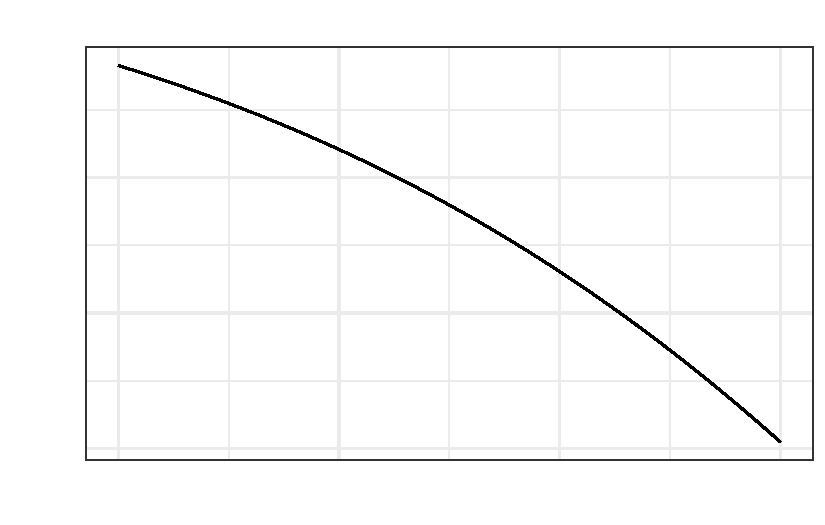
\includegraphics{main_files/figure-pdf/fig-line-plot-1.pdf}

}

\caption{\label{fig-line-plot}Probabilidade de não fumar}

\end{figure}

\begin{Shaded}
\begin{Highlighting}[]
\FunctionTok{ggplot}\NormalTok{(new\_df, }\FunctionTok{aes}\NormalTok{(}\AttributeTok{x =}\NormalTok{ distorcao\_idade\_serie, }\AttributeTok{y =}\NormalTok{ fit}\FloatTok{.2}\NormalTok{)) }\SpecialCharTok{+} \FunctionTok{geom\_line}\NormalTok{() }\SpecialCharTok{+} \FunctionTok{labs}\NormalTok{(}\AttributeTok{title =} \StringTok{"Probabilidade de fumar 1 ou 2 dias"}\NormalTok{, }\AttributeTok{y =} \StringTok{"Probabilidade"}\NormalTok{, }\AttributeTok{x =} \StringTok{"Distorção idade{-}série"}\NormalTok{) }\SpecialCharTok{+}\NormalTok{ abnt\_theme}
\end{Highlighting}
\end{Shaded}

\begin{figure}[H]

{\centering 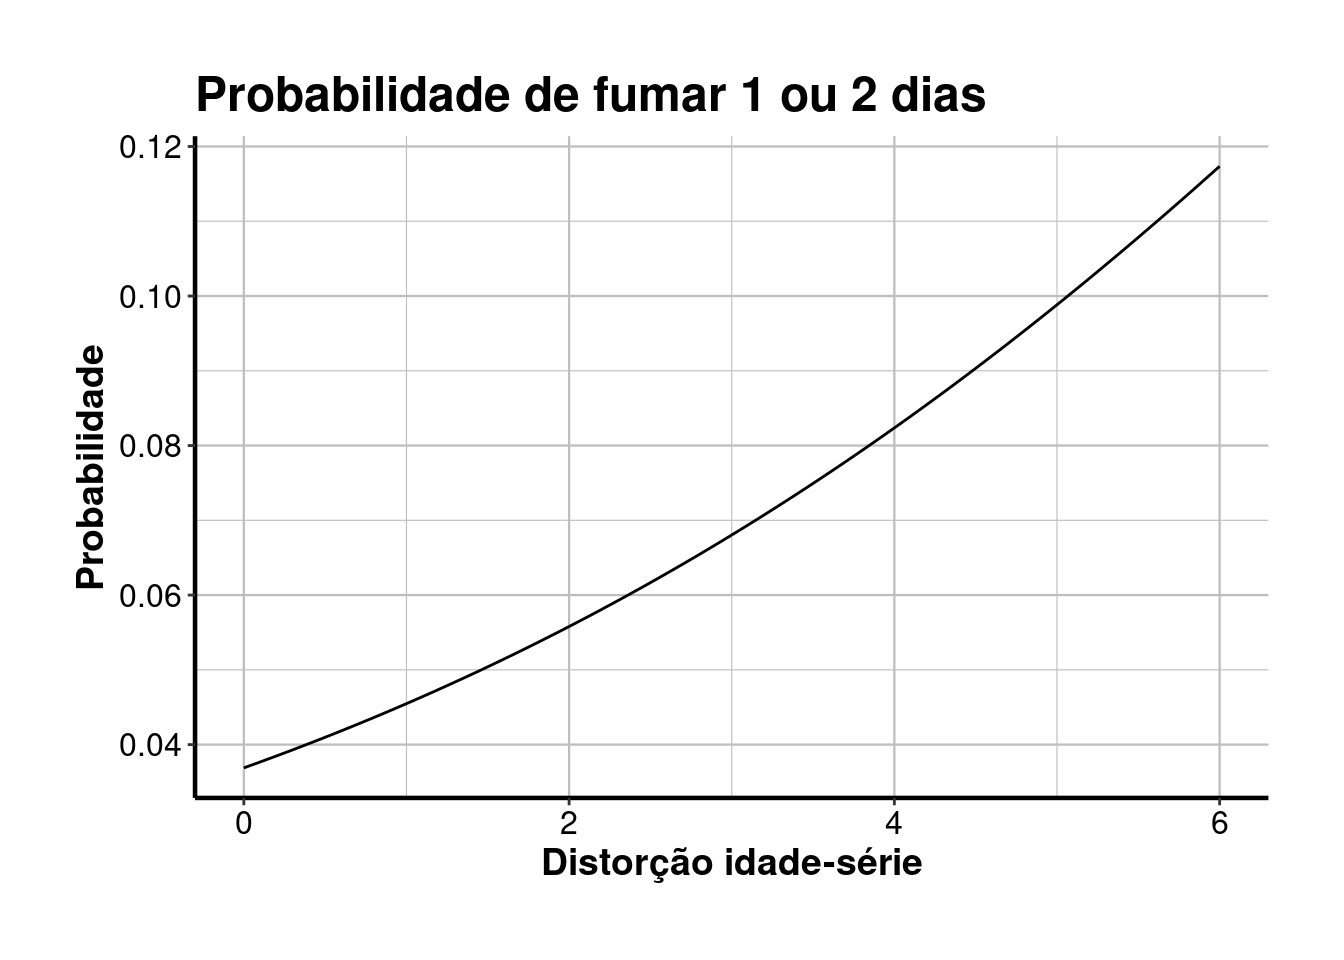
\includegraphics{main_files/figure-pdf/fig-line-plot2-1.pdf}

}

\caption{\label{fig-line-plot2}Probabilidade de fumar 1 ou 2 dias}

\end{figure}

\begin{Shaded}
\begin{Highlighting}[]
\FunctionTok{ggplot}\NormalTok{(new\_df, }\FunctionTok{aes}\NormalTok{(}\AttributeTok{x =}\NormalTok{ distorcao\_idade\_serie, }\AttributeTok{y =}\NormalTok{ fit}\FloatTok{.3}\NormalTok{)) }\SpecialCharTok{+} \FunctionTok{geom\_line}\NormalTok{() }\SpecialCharTok{+} \FunctionTok{labs}\NormalTok{(}\AttributeTok{title =} \StringTok{"Probabilidade de fumar 3 a 5 dias"}\NormalTok{, }\AttributeTok{y =} \StringTok{"Probabilidade"}\NormalTok{, }\AttributeTok{x =} \StringTok{"Distorção idade{-}série"}\NormalTok{) }\SpecialCharTok{+}\NormalTok{ abnt\_theme}
\end{Highlighting}
\end{Shaded}

\begin{figure}[H]

{\centering 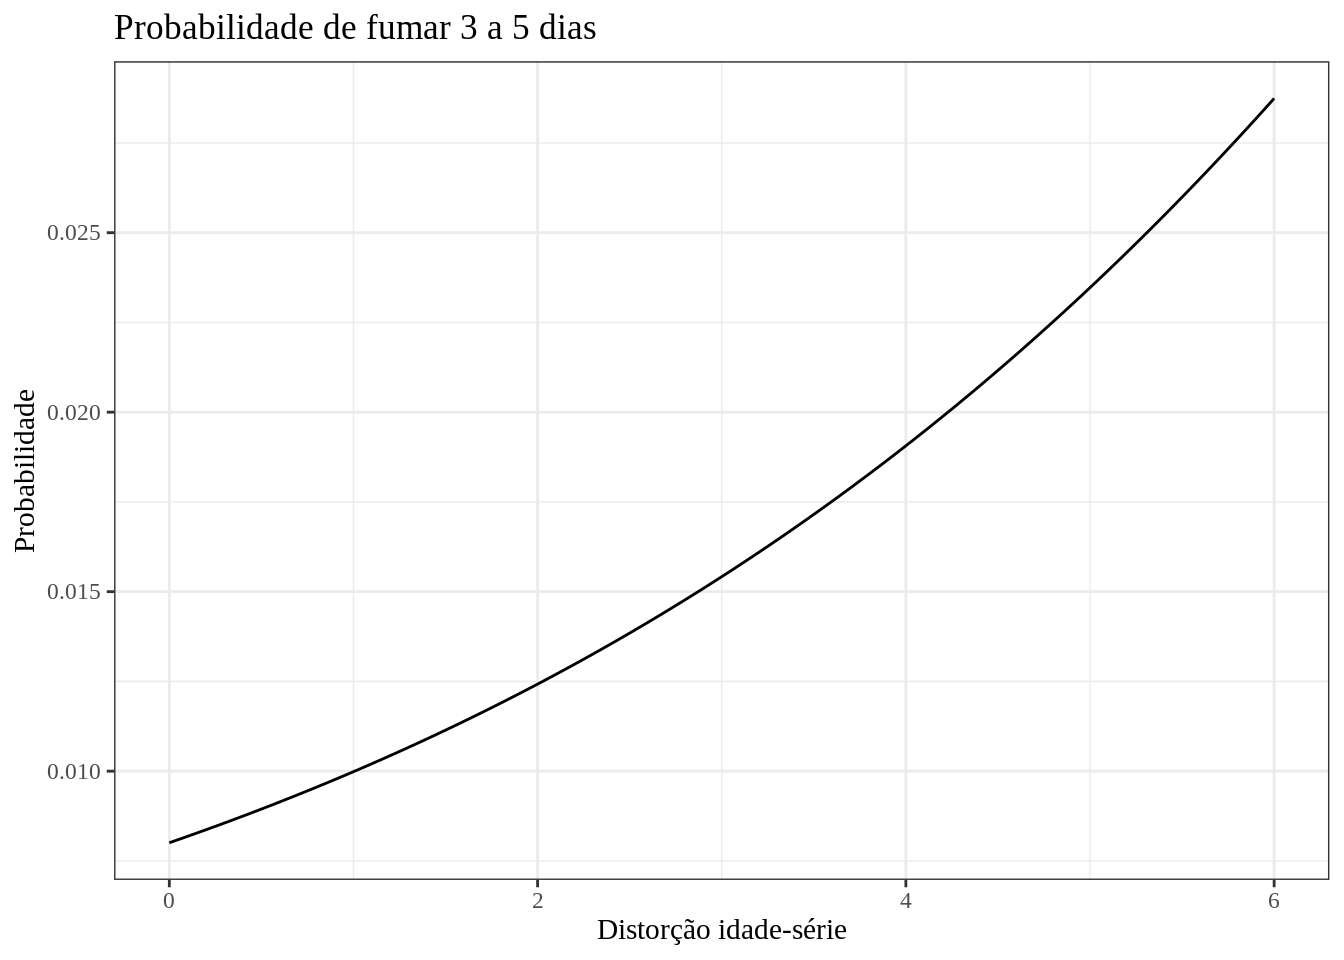
\includegraphics{main_files/figure-pdf/fig-line-plot3-1.pdf}

}

\caption{\label{fig-line-plot3}Probabilidade de fumar 3 a 5 dias}

\end{figure}

\begin{Shaded}
\begin{Highlighting}[]
\FunctionTok{ggplot}\NormalTok{(new\_df, }\FunctionTok{aes}\NormalTok{(}\AttributeTok{x =}\NormalTok{ distorcao\_idade\_serie, }\AttributeTok{y =}\NormalTok{ fit}\FloatTok{.4}\NormalTok{)) }\SpecialCharTok{+} \FunctionTok{geom\_line}\NormalTok{() }\SpecialCharTok{+} \FunctionTok{labs}\NormalTok{(}\AttributeTok{title =} \StringTok{"Probabilidade de fumar 6 a 9 dias"}\NormalTok{, }\AttributeTok{y =} \StringTok{"Probabilidade"}\NormalTok{, }\AttributeTok{x =} \StringTok{"Distorção idade{-}série"}\NormalTok{) }\SpecialCharTok{+}\NormalTok{ abnt\_theme}
\end{Highlighting}
\end{Shaded}

\begin{figure}[H]

{\centering 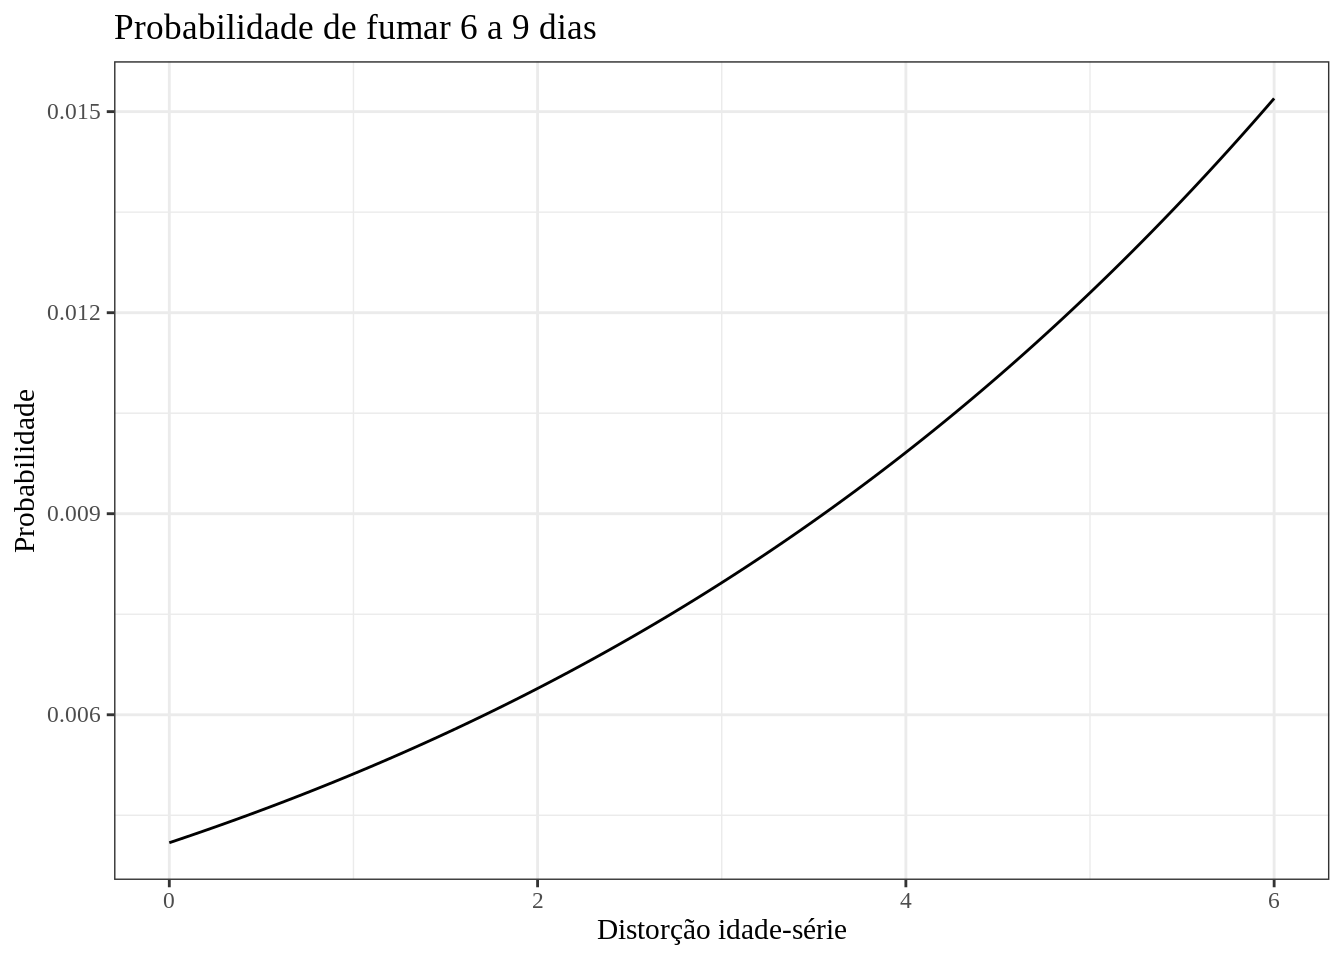
\includegraphics{main_files/figure-pdf/fig-line-plot4-1.pdf}

}

\caption{\label{fig-line-plot4}Probabilidade de fumar 6 a 9 dias}

\end{figure}

\begin{Shaded}
\begin{Highlighting}[]
\FunctionTok{ggplot}\NormalTok{(new\_df, }\FunctionTok{aes}\NormalTok{(}\AttributeTok{x =}\NormalTok{ distorcao\_idade\_serie, }\AttributeTok{y =}\NormalTok{ fit}\FloatTok{.5}\NormalTok{)) }\SpecialCharTok{+} \FunctionTok{geom\_line}\NormalTok{() }\SpecialCharTok{+} \FunctionTok{labs}\NormalTok{(}\AttributeTok{title =} \StringTok{"Probabilidade de fumar 10 a 19 dias"}\NormalTok{, }\AttributeTok{y =} \StringTok{"Probabilidade"}\NormalTok{, }\AttributeTok{x =} \StringTok{"Distorção idade{-}série"}\NormalTok{) }\SpecialCharTok{+}\NormalTok{ abnt\_theme}
\end{Highlighting}
\end{Shaded}

\begin{figure}[H]

{\centering 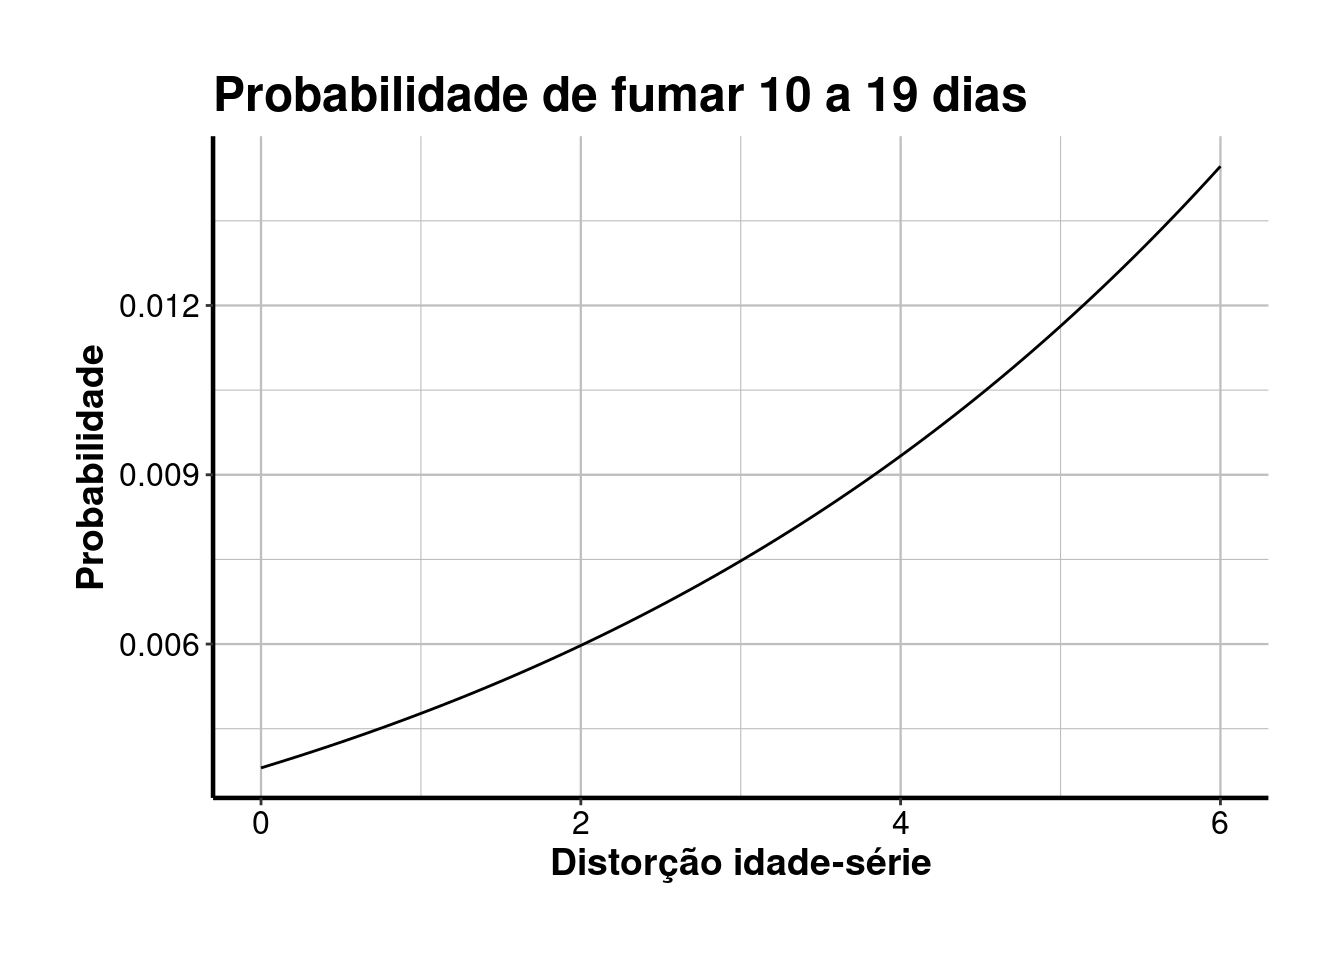
\includegraphics{main_files/figure-pdf/fig-line-plot5-1.pdf}

}

\caption{\label{fig-line-plot5}Probabilidade de fumar 10 a 19 dias}

\end{figure}

\begin{Shaded}
\begin{Highlighting}[]
\FunctionTok{ggplot}\NormalTok{(new\_df, }\FunctionTok{aes}\NormalTok{(}\AttributeTok{x =}\NormalTok{ distorcao\_idade\_serie, }\AttributeTok{y =}\NormalTok{ fit}\FloatTok{.6}\NormalTok{)) }\SpecialCharTok{+} \FunctionTok{geom\_line}\NormalTok{() }\SpecialCharTok{+} \FunctionTok{labs}\NormalTok{(}\AttributeTok{title =} \StringTok{"Probabilidade de fumar 20 a 29 dias"}\NormalTok{, }\AttributeTok{y =} \StringTok{"Probabilidade"}\NormalTok{, }\AttributeTok{x =} \StringTok{"Distorção idade{-}série"}\NormalTok{) }\SpecialCharTok{+}\NormalTok{ abnt\_theme}
\end{Highlighting}
\end{Shaded}

\begin{figure}[H]

{\centering 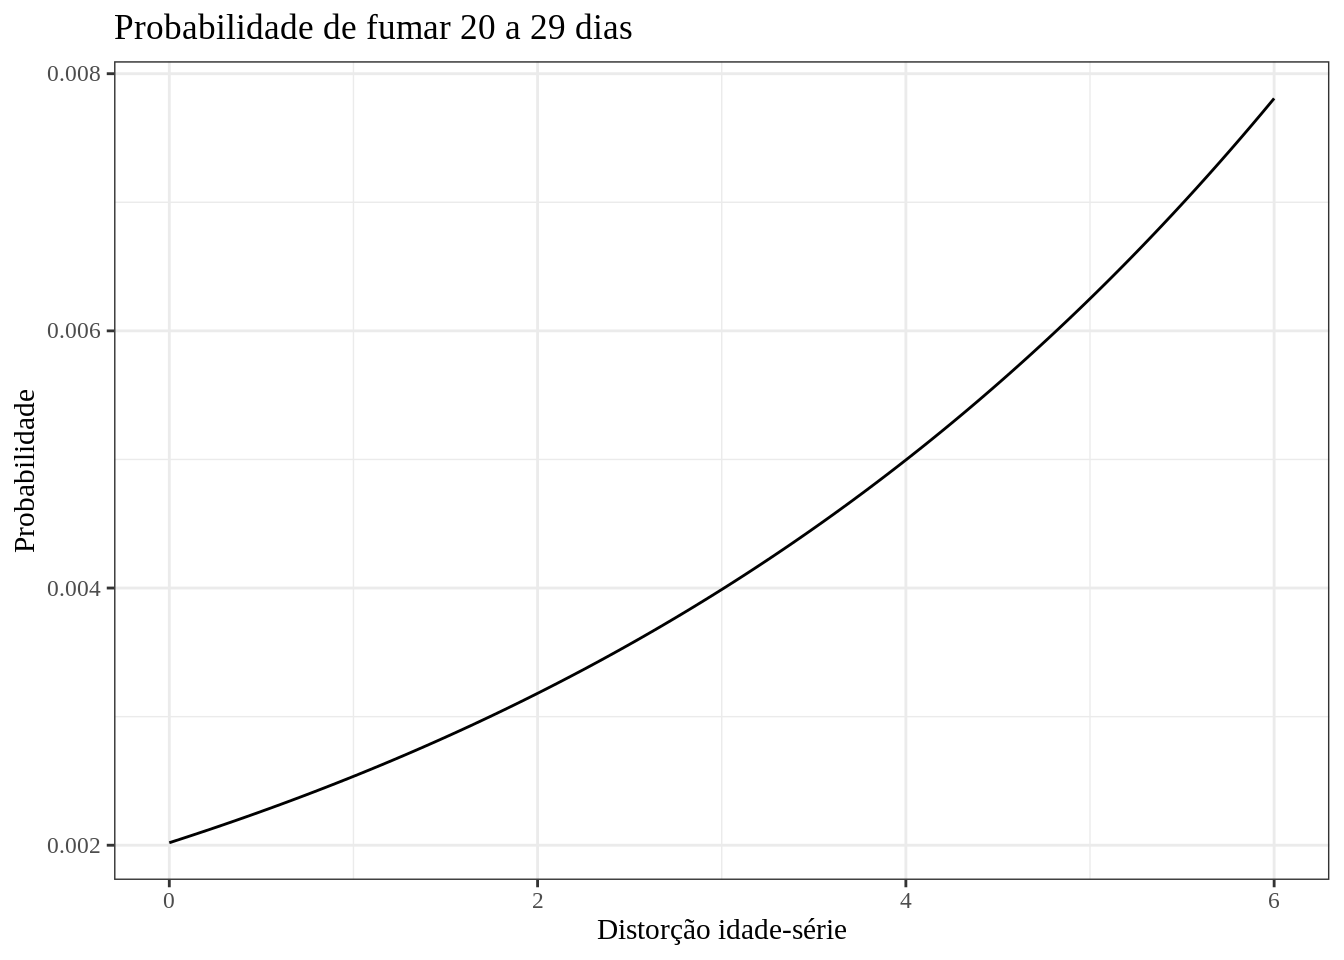
\includegraphics{main_files/figure-pdf/fig-line-plot6-1.pdf}

}

\caption{\label{fig-line-plot6}Probabilidade de fumar 20 a 29 dias}

\end{figure}

\begin{Shaded}
\begin{Highlighting}[]
\FunctionTok{ggplot}\NormalTok{(new\_df, }\FunctionTok{aes}\NormalTok{(}\AttributeTok{x =}\NormalTok{ distorcao\_idade\_serie, }\AttributeTok{y =}\NormalTok{ fit}\FloatTok{.7}\NormalTok{)) }\SpecialCharTok{+} \FunctionTok{geom\_line}\NormalTok{() }\SpecialCharTok{+} \FunctionTok{labs}\NormalTok{(}\AttributeTok{title =} \StringTok{"Probabilidade de fumar todos os dias"}\NormalTok{, }\AttributeTok{y =} \StringTok{"Probabilidade"}\NormalTok{, }\AttributeTok{x =} \StringTok{"Distorção idade{-}série"}\NormalTok{) }\SpecialCharTok{+}\NormalTok{ abnt\_theme}
\end{Highlighting}
\end{Shaded}

\begin{figure}[H]

{\centering 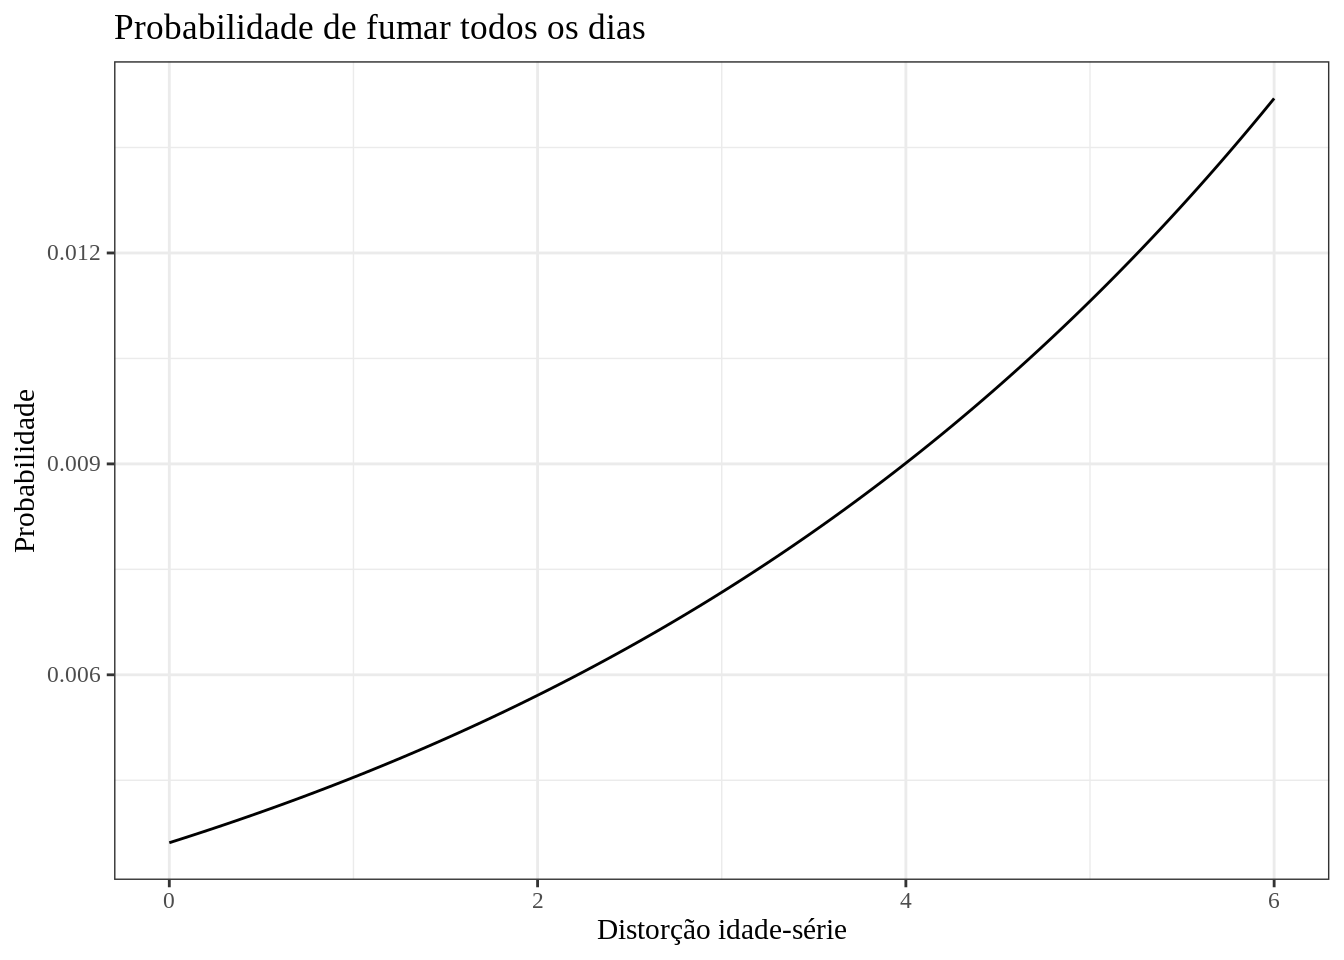
\includegraphics{main_files/figure-pdf/fig-line-plot7-1.pdf}

}

\caption{\label{fig-line-plot7}Probabilidade de fumar todos os dias}

\end{figure}

\hypertarget{referuxeancias}{%
\subsubsection{Referências}\label{referuxeancias}}

\hypertarget{refs}{}
\begin{CSLReferences}{0}{1}
\leavevmode\vadjust pre{\hypertarget{ref-agresti}{}}%
AGRESTI, A. \textbf{Categorical data analysis, Second Edition}. New
York, New York: Wiley, 2002.

\leavevmode\vadjust pre{\hypertarget{ref-bousquet}{}}%
BOUSQUET, C. A. H. et al.
\href{https://doi.org/10.1163/1568539X-00003431}{Determinants of
leadership in groups of female mallards}. \textbf{Behaviour}, v. 154, n.
4, p. 467--507, 2017.

\leavevmode\vadjust pre{\hypertarget{ref-christensen}{}}%
CHRISTENSEN, R. H. B. \textbf{ordinal --- Regression models for ordinal
data}. Disponível em:
\textless{}\url{http://www.cran.r-project.org/package=ordinal/}\textgreater.

\leavevmode\vadjust pre{\hypertarget{ref-oconnell}{}}%
O'CONNELL, A. A. \textbf{An illustration of multilevel models for
ordinal response data}. Data and context in statistics education:
Towards an evidence-based society. Proceedings of the Eighth
International Conference on Teaching Statistics (ICOTS8).
\textbf{Anais}...2010.

\leavevmode\vadjust pre{\hypertarget{ref-raudenbush}{}}%
RAUDENBUSH, S. W.; BRYK, A. S. \textbf{Hierarchical linear models:
Applications and data analysis methods}. {[}s.l.{]} sage, 2002. v. 1

\end{CSLReferences}



\end{document}
